\chapter{Fast and Expressive Anonymous Credentials from New Rerandomizable Signatures}\label{chap2}


\subsection{Motivation}

Digital interactions are shifting toward the self‑sovereign identity (SSI) model, where users control cryptographic credentials in digital wallets. In this paradigm, a wallet is not just a storage container, but a user-controlled agent for issuing, holding, and presenting zero-knowledge proofs of credentials across interoperable systems. Governments and industry are mandating digital wallets (e.g., EU Digital Wallet Regulation \cite{noauthor_regulation_2024}; 13 U.S. jurisdictions issuing mobile driver’s licenses \cite{aamva_jurisdiction_nodate}). Credential Oracles \cite{zhang_deco_2020, celi_distefano_2025} are "feeder services" that generate verifiable data attestations from different sources such as Web 2.0 credentials, bank data, or offline information.  The digital attestations are associated with a user's credential wallet and stored "within" the wallet. Commodity devices—from smartphones to IoT sensors—will sign outputs (photos, logs, transactions) with device keys (e.g., C2PA \cite{c2paorg_content_2024}), turning everyday interactions into verifiable claims. As AI-generated media and deepfakes proliferate, cryptographic provenance becomes critical, exponentially increasing the volume and heterogeneity of credentials that wallets must manage.


Previous deployments of Anonymous Credentials like IBM's Idemix \cite{camenisch_design_2002} and IRMA \cite{fischer-hubner_towards_2013} based on CL-Signatures \cite{camenisch_design_2002, cimato_signature_2003}, Hyperledger Fabric \cite{androulaki_hyperledger_2018} based on BBS+ \cite{hutchison_constant-size_2006}, Microsoft's U-Prove \cite{dunkelman_formal_2016} based on Brands' signatures \cite{brands_rethinking_2000}, were deployed in pilot programs \cite{dunkelman_formal_2016}, and proved that these systems were secure, private and feature-rich, but inefficient for widespread adoption. Their implementations were based on early constructions we label as "previous generation" and lacked efficient credential verification procedures required for the expected user experience needed for large-scale uptake, which we illustrate below.

% The performance comparison in Table \ref{tab:anon_creds_performance_old_gen_vs_new} demonstrates that newer anonymous credential schemes, such as BBS+2016 \cite{camenisch_anonymous_2016} and PS-UTT22 \cite{tomescu_utt_2022}, outperform older schemes like BBS+06 \cite{hutchison_constant-size_2006} and PS16 \cite{sako_short_2016} by shifting zero-knowledge proofs from the target group $(\mathbb{G}_T)$ to the source group ($\mathbb{G}_1)$\footnote{CL04 \cite{hutchison_signature_2004} is included in previous generation}. For 30 attributes, older schemes require computing over 3$\ell$, and 2$\ell$ $\G_T$ points respectively with Show and Verify times of 39.21 ms (BBS+06) and 32.78 ms (PS16). In comparison, newer schemes compute only in $\G_1$ and minimize pairings, achieving times of 5.72 ms and 5.38 ms—speedups of 6.85x and 6.09x, respectively. These improvements maintain full functionality, including selective disclosure and unlinkability, and rely on standard security assumptions, enhancing the practicality of anonymous credentials for digital identity systems.





\subsection{Problems and Scope}

The proliferation of credential types, sources, and volume reveals three gaps in existing schemes:

\begin{enumerate}
   \item \textbf{Scalability for wallet-centric architectures.} In the SSI model, wallets will accumulate potentially thousands of heterogeneous credentials (identity documents, transaction receipts, device-signed content, oracle attestations). Presentation must remain succinct even in scenarios where proof aggregation is possible.

    \item \textbf{Security against untrusted issuers.} The decentralized ecosystem includes credential oracles, device-embedded signers, and third-party attesters with varying security assumptions. User privacy (unlinkability, anonymity) must hold even when issuers collude or behave arbitrarily, protecting users from tracking by malicious ecosystem participants.

    \item \textbf{Expressive, efficient zero-knowledge proofs.} Users need to prove dynamic policies over attribute sets (e.g., "prove I'm over 18 AND in EU AND my device captured this photo today"). Achieving rich predicate support beyond simple possession proofs, without heavy SNARK primitives, is essential for mobile device feasibility.

\end{enumerate}

Solving these challenges requires a foundational understanding of how anonymous credentials evolved to address similar scalability and security concerns. While existing systems have made significant progress, none fully address the demands of the SSI wallet-centric ecosystem we've described. To build this next-generation system, we must first examine the architectural decisions and cryptographic innovations that brought us to this point.

Anonymous credentials are a fundamental building block for privacy-preserving digital identity, aligning perfectly with the SSI principle that users should prove attributes without revealing full identity. Since their first inception by Chaum \cite{chaum_untraceable_1981}, they have evolved from theoretical constructs to practical systems deployed in real-world applications such as U-Prove, Idemix, and PrivacyPass \cite{camenisch_design_2002, dunkelman_formal_2016}, but none have been designed explicitly for wallet-centric architectures managing thousands of heterogeneous credentials. 

Despite these advances, current ABC systems face critical gaps that prevent wide-scale deployment in the SSI ecosystem we've outlined.  Systems like SPS-EQ \cite{fuchsbauer_structure-preserving_2019, hanaoka_improved_2022} and ACT \cite{guo_anonymous_2023} achieve high efficiency but support only limited predicates, while approaches based on zkSNARKs enable rich expressiveness \cite{rosenberg_zk-creds_2022} but at computational cost. Furthermore, many anonymous credential systems assume honest issuers, leaving users vulnerable to privacy breaches from malicious credential providers, especially when issuers might be credential oracles.

This chapter develops the cryptographic foundations needed for credential wallets. We address each of the identified challenges through four key contributions that together enable efficient, secure, and expressive anonymous credentials at the scale demanded by the SSI ecosystem:

\begin{enumerate}
    \item \textbf{Complete Security Proofs for an efficient PS signature variant from UTT:} We provide formal security proofs that were only sketched in \cite{tomescu_utt_2022}:
    \begin{itemize}
        \item Position-binding vector commitments under SDLP in the Algebraic Group Model (Section \ref{sec:commitment})
        \item EUF-CMA security for rerandomizable signatures over commitments under PS-LRSW (Section \ref{sec:formal_treatment_utt_rerand_sig})
        \item Satisfaction of Anonymous Credential model \cite{fuchsbauer_structure-preserving_2019} security properties—correctness, unforgeability, and anonymity—for multi-show operations (Section \ref{sec:abc})
    \end{itemize}

    \item \textbf{Fastest Show+Verify Operations:} Our construction achieves 10-16\% faster verification than UTT \cite{tomescu_utt_2022} and outperforms the most popular BBS+ variant \cite{camenisch_anonymous_2016} - we validate through comprehensive benchmarks \ref{sec:performance_evaluation}.

    \item \textbf{Malicious Issuer Security through Key Verification Protocols:} We formalize anonymity guarantees against malicious issuer via mandatory key verification (Section \ref{subsec:malicious_issuer_security_guarantee}), preventing deanonymization attacks through maliciously generated keys—a vulnerability that existing schemes do not address.

    \item \textbf{Empirical Validation of Schnorr Protocol Efficiency:} Comprehensive benchmarks \ref{fig:schnorr-benchmarks}reveal that Schnorr protocols achieve sublinear complexity for attribute proofs via multi-scalar multiplication, outperforming theoretical predictions and enabling almost constant-size expressive predicate evaluation.
\end{enumerate}

\subsubsection*{Chapter Roadmap}
This chapter develops cryptographic foundations for efficient anonymous credentials in decentralized identity systems. Section \ref{chap2:preliminaries} establishes our mathematical setting with SDLP and PS-LRSW assumptions.

Section \ref{sec:formal_treatment_utt_rerand_sig} provides the first complete security proofs for our rerandomizable signature scheme, proving position-binding under SDLP and EUF-CMA security under PS-LRSW. Section \ref{chap2:extending_utt_construction} presents our key optimization: moving signatures from $\G_1$ to $\G_2$ for 10-16\% faster verification, plus malicious issuer protection through key verification.

Section \ref{chap2:expressive_proofs} demonstrates how Sigma protocols achieve efficient predicate evaluation over complex policies. Section \ref{sec:abc} constructs our complete credential system with security proofs. Section \ref{sec:performance_evaluation} validates our approach through benchmarks, showing state-of-the-art performance with up to 83\% verification speedup.






\section{Preliminaries}\label{chap2:preliminaries}


\subsection{Assumptions}


\begin{definition}[Symmetric Discrete Logarithm Assumption (SDLP)]\label{sdlp}
For any PPT adversary $\mathcal{A}$, we say the SDLP assumption holds if there exists a negligible function $\negl$ such that:
$$\Pr\left[\begin{array}{l}
    \BG = (p, \G_1, \G_2, \G_T, e, g, \tilde{g}) \sample \BGGen(1^\lambda) \\
    x \sample \Z_p \\
    x' \sample \mathcal{A}(\BG, g^x, \tilde{g}^x)
\end{array} : x = x'\right] \leq \negl(\lambda)$$
where validity of input can be verified by checking $e(g, \tilde{g}^x) = e(g^x, \tilde{g})$.
\end{definition} 


\begin{definition}[Type-3 PS-LRSW Assumption]
For any PPT adversary $\mathcal{A}$, we say the Type-3 PS-LRSW assumption holds in the generic bilinear group model if there exists a negligible function $\negl$ such that:
$$\Pr\left[\begin{array}{l}
    \BG = (p, \G_1, \G_2, \G_T, e, g, \tilde{g}) \sample \BGGen(1^\lambda) \\
    x,y \sample \Z_p, X \gets g^x, \tilde{X} \gets \tilde{g}^x, \tilde{Y} \gets \tilde{g}^y \\
    (m^*, P_1, P_2) \sample \mathcal{A}^{\mathcal{O}_{x,y}}(\BG, X, \tilde{Y})
\end{array} : \begin{array}{l}
    m^* \notin Q \land P_1 \neq 1_{\G_1} \land \\
    e(P_1, \tilde{X} \cdot \tilde{Y}^{m^*}) = e(P_2, \tilde{g})
\end{array}\right] \leq \negl$$
where $Q$ is the set of queries made to $\mathcal{O}_{x,y}$ with access to $x,y$ is defined by:
\[
\text{Oracle }\mathcal{O}_{x,y}(m): \text{ Samples } h \sample \G_1, \text{ Returns the pair } P = (h, h^{x+my})
\]

\end{definition}






\subsection{Dual-Group Pedersen Commitments}\label{sec:commitment}
In this section, we introduce a specialized extension of Pedersen commitments that supports vector messages, rerandomizability, and position binding. Our main contribution is a security proof in the Algebraic Group Model (AGM) that establishes position binding based on the Symmetric Discrete Logarithm Problem (SDLP).


\begin{definition}[Commitment Scheme]\label{def:commitmentscheme}
A commitment scheme $\mathsf{Com}$ is a tuple of probabilistic polynomial-time algorithms $(\mathsf{Setup}, \mathsf{Commit}, \mathsf{Open})$ where:
\begin{itemize}
    \item $\mathsf{Setup}(1^\lambda) \rightarrow \mathsf{ck}$: is a probabilistic algorithm that takes as input a security parameter $\lambda$ and outputs a commitment key $\mathsf{ck}$. The message space $\mathcal{M}$ is implicitly defined by $\mathsf{ck}$.
    
    \item $\mathsf{Commit}(\mathsf{ck}, m) \rightarrow (\mathsf{cm}, r)$: is a probabilistic algorithm that takes as input the commitment key $\mathsf{ck}$ and a message $m \in \mathcal{M}$. It outputs a commitment $\mathsf{cm}$ and an opening value $r$.
    
    \item $\mathsf{Open}(\mathsf{ck}, \mathsf{cm}, m, r) \rightarrow b$: is a deterministic algorithm that takes as input the commitment key $\mathsf{ck}$, a commitment $\mathsf{cm}$, a message $m$, and an opening value $r$. It outputs a bit $b \in \{0,1\}$, where 1 indicates a valid opening and 0 indicates an invalid opening.
\end{itemize}
\end{definition}

\begin{definition}[Correctness]
A commitment scheme $(\mathsf{Setup}, \mathsf{Commit}, \mathsf{Open})$ is correct if for all $\lambda \in \mathbb{N}$, all commitment keys $\mathsf{ck} \in [\mathsf{Setup}(1^\lambda)]$, and all messages $m \in \mathcal{M}$:
$$\Pr[(\mathsf{cm}, r) \sample \mathsf{Commit}(\mathsf{ck}, m) : \mathsf{Open}(\mathsf{ck}, \mathsf{cm}, m, r) = 1] = 1.$$
\end{definition}

\begin{definition}[Hiding]
A commitment scheme $(\mathsf{Setup}, \mathsf{Commit}, \mathsf{Open})$ is hiding if for all PPT adversaries $\mathcal{A}$, there exists a negligible function $\negl$ such that:
$$\left|\Pr\left[\begin{array}{l}
    \mathsf{ck} \sample \mathsf{Setup}(1^\lambda) \\
    (m_0, m_1) \sample \mathcal{A}(\mathsf{ck}) \\
    b \sample \{0,1\} \\
    (\mathsf{cm}, r) \sample \mathsf{Commit}(\mathsf{ck}, m_b) \\
    b' \sample \mathcal{A}(\mathsf{ck}, \mathsf{cm})
\end{array} : b' = b\right] - \frac{1}{2}\right| \leq \negl(\lambda)$$
\end{definition}

\begin{definition}[Binding]
A commitment scheme $(\mathsf{Setup}, \mathsf{Commit}, \mathsf{Open})$ is binding if for all PPT adversaries $\mathcal{A}$, there exists a negligible function $\negl$ such that:
$$\Pr\left[\begin{array}{l}
    \mathsf{ck} \sample \mathsf{Setup}(1^\lambda) \\
    (\mathsf{cm}, m_0, m_1, r_0, r_1) \sample \mathcal{A}(\mathsf{ck})
\end{array} : \begin{array}{l}
    m_0 \neq m_1 \land \\
    \mathsf{Open}(\mathsf{ck}, \mathsf{cm}, m_0, r_0) = 1 \land \\
    \mathsf{Open}(\mathsf{ck}, \mathsf{cm}, m_1, r_1) = 1
\end{array}\right] \leq \negl(\lambda)$$
\end{definition}



\subsubsection{Dual-Group Construction for Vector of Messages}

We instantiate a rerandomizable commitment scheme to a vector of messages in the bilinear group setting as per the construction in \cite{tomescu_utt_2022} to enable efficient integration with our signature scheme. Let $\G_1, \G_2$ be cyclic groups of prime order $p$ with an efficient Type-3 pairing $e: \G_1 \times \G_2 \to \G_T$.

\begin{itemize}
    \item $\mathsf{Setup}(1^\lambda, 1^n) \to \mathsf{ck}$:
    Sample generators $(g, \tilde{g}) \sample \G_1 \times \G_2$.
    For $i \in [1,n]$: Sample $y_i \sample \Z_p$, compute $(g_i, \tilde{g}_i) \gets (g^{y_i}, \tilde{g}^{y_i})$.
    Return $\mathsf{ck} \gets (g, (g_1,\ldots,g_n), \tilde{g}, (\tilde{g}_1,\ldots,\tilde{g}_n))$.
    
    \item $\mathsf{Commit}(\mathsf{ck}, \attrs) \to (\mathsf{cm}, \widetilde{\mathsf{cm}}, r)$:
    Parse $\mathsf{ck}$ as $(g, (g_1,\ldots,g_n), \tilde{g}, (\tilde{g}_1,\ldots,\tilde{g}_n))$.
    Sample $r \sample \Z_p$.
    Compute $\mathsf{cm} \gets g^r \prod_{i=1}^n g_i^{m_i}$ and $\widetilde{\mathsf{cm}} \gets \tilde{g}^r \prod_{i=1}^n \tilde{g}_i^{m_i}$.
    Return $(\mathsf{cm}, \widetilde{\mathsf{cm}}, r)$.
    
    \item $\mathsf{Open}(\mathsf{ck}, (\mathsf{cm}, \widetilde{\mathsf{cm}}), \attrs, r) \to \{0,1\}$:
    Check if $\mathsf{cm} = g^r \prod_{i=1}^n g_i^{m_i}$ and $\widetilde{\mathsf{cm}} = \tilde{g}^r \prod_{i=1}^n \tilde{g}_i^{m_i}$.
    Additionally, verify $e(\mathsf{cm}, \tilde{g}) = e(g, \widetilde{\mathsf{cm}})$.
    Return 1 if all checks pass, 0 otherwise.
    
    \item $\mathsf{Rerand}(\mathsf{ck}, (\mathsf{cm}, \widetilde{\mathsf{cm}}), \Delta_r) \to ({\mathsf{cm}}', \widetilde{\mathsf{cm}}', r')$:
    Compute ${\mathsf{cm}}' \gets \mathsf{cm} \cdot g^{\Delta_r}$ and $\widetilde{\mathsf{cm}}' \gets \widetilde{\mathsf{cm}} \cdot \tilde{g}^{\Delta_r}$.
    Set $r' \gets r + \Delta_r$.
    Return $({\mathsf{cm}}', \widetilde{\mathsf{cm}}', r')$.
\end{itemize}

This construction preserves the message vector while updating the randomness, making rerandomized commitments computationally indistinguishable from fresh commitments to the same message.









\subsection{Rerandomizable Signature over Commitments}\label{sec:rerandsig_commitment}



\begin{definition}[Signature Scheme]
A signature scheme $\mathsf{Sig}$ is a tuple of probabilistic polynomial-time algorithms $(\mathsf{KeyGen}, \mathsf{Sign}, \mathsf{Verify})$ where:

\begin{itemize}
    \item $\mathsf{KeyGen}(1^\lambda) \rightarrow (\mathsf{sk}, \mathsf{pk})$: is a probabilistic algorithm that takes as input a security parameter $\lambda$ and outputs a secret signing key $\mathsf{sk}$ and a public verification key $\mathsf{pk}$. The message space $\mathcal{M}$ is implicitly defined by $\mathsf{pk}$.
    
    \item $\mathsf{Sign}(\mathsf{sk}, m; r) \rightarrow \sigma$: is a probabilistic algorithm that takes as input the secret key $\mathsf{sk}$, a message $m \in \mathcal{M}$, and random coins $r$ sampled from the randomness space $\mathcal{R}$. It outputs a signature $\sigma$.
    
    \item $\mathsf{Verify}(\mathsf{pk}, m, \sigma) \rightarrow b$: is a deterministic algorithm that takes as input the public key $\mathsf{pk}$, a message $m \in \mathcal{M}$, and a signature $\sigma$. It outputs a bit $b \in \{0,1\}$, where 1 indicates acceptance and 0 indicates rejection.
\end{itemize}
\end{definition}

\begin{definition}[Correctness]
A signature scheme $(\mathsf{KeyGen}, \mathsf{Sign}, \mathsf{Verify})$ is correct if for all $k \in \mathbb{N}$, all key pairs $(\mathsf{sk}, \mathsf{pk}) \in [\mathsf{KeyGen}(1^k)]$ and all $m \in \mathcal{M}$ we have:

$$\Pr[\mathsf{Verify}(m, \mathsf{Sign}(m, \mathsf{sk}), \mathsf{pk}) = 1] = 1.$$
\end{definition}

\begin{definition}[EUF-CMA Security]
A signature scheme $(\mathsf{KeyGen}, \mathsf{Sign}, \mathsf{Verify})$ is existentially unforgeable under adaptive chosen-message attacks if for all PPT algorithms $\mathcal{A}$, there exists a negligible function $\negl$ such that:
$$\Pr\left[\begin{array}{l}
    (\mathsf{sk}, \mathsf{pk}) \sample \mathsf{KeyGen}(1^\lambda) \\
    (m^*, \sigma^*) \sample \mathcal{A}^{\mathcal{O}_{\mathsf{sk}}}(\mathsf{pk})
\end{array} : \begin{array}{l}
    m^* \notin Q \land \\
    \mathsf{Verify}(m^*, \sigma^*, \mathsf{pk}) = 1
\end{array}\right] \leq \negl$$
where $Q$ is the set of queries made to $\mathcal{O}_{\mathsf{sk}}$ with access to $\mathsf{sk}$ is defined by:
\[
\text{Oracle }\mathcal{O}_{\mathsf{sk}}(m): \text{ Returns } \sigma \gets \mathsf{Sign}(m, \mathsf{sk})
\]
\end{definition}




\begin{definition}[Rerandomizable Signature]
A rerandomizable signature scheme over commitments $\mathsf{RS}$ extends a standard signature scheme with the following interface:
\begin{itemize}
    \item $\mathsf{KeyGen}(1^\lambda, \mathsf{ck}) \rightarrow (\mathsf{sk}, \mathsf{pk})$: Takes security parameter $\lambda$ and commitment key $\mathsf{ck}$, outputs signing key $\mathsf{sk}$ and verification key $\mathsf{pk}$.
    
    \item $\mathsf{Sign}(\mathsf{sk}, \mathsf{cm}; u) \rightarrow \sigma$: Signs commitment $\mathsf{cm}$ using signing key $\mathsf{sk}$ and randomness $u$.
    
    \item $\mathsf{Rerand}(\mathsf{pk}, \sigma, \Delta_r, \Delta_u) \rightarrow \sigma'$: Creates a rerandomized signature $\sigma'$ from signature $\sigma$ using randomization values $\Delta_r, \Delta_u$.
    
    \item $\mathsf{Verify}(\mathsf{pk}, \mathsf{cm}, \sigma) \rightarrow \{0,1\}$: Verifies signature $\sigma$ on commitment $\mathsf{cm}$ using public key $\mathsf{pk}$.
\end{itemize}
\end{definition}

\begin{definition}[Correctness]
A rerandomizable signature scheme over commitments satisfies correctness if for all security parameters $\lambda$, all key pairs $(\mathsf{sk}, \mathsf{pk}) \in [\mathsf{KeyGen}(1^\lambda, \mathsf{ck})]$, all messages $m \in \mathcal{M}$, all valid commitments $\mathsf{cm} = \mathsf{CM.Commit}(\mathsf{ck}, m, r)$, and all randomness values $u, \Delta_r, \Delta_u$:

\begin{enumerate}
    \item \textbf{Basic Verification}: $\mathsf{Verify}(\mathsf{pk}, \mathsf{cm}, \mathsf{Sign}(\mathsf{sk}, \mathsf{cm}; u)) = 1$
    
    \item \textbf{Rerandomization Consistency}: $\mathsf{Verify}(\mathsf{pk}, \mathsf{CM.Rerand}(\mathsf{ck}, \mathsf{cm}, \Delta_r), \mathsf{Rerand}(\mathsf{pk}, \sigma, \Delta_r, \Delta_u)) = 1$ where $\sigma = \mathsf{Sign}(\mathsf{sk}, \mathsf{cm}; u)$
    
    \item \textbf{Rerandomization Equivalence}: The distribution of $\mathsf{Rerand}(\mathsf{pk}, \mathsf{Sign}(\mathsf{sk}, \mathsf{cm}; u), \Delta_r, \Delta_u)$ is computationally indistinguishable from $\mathsf{Sign}(\mathsf{sk}, \mathsf{CM.Rerand}(\mathsf{ck}, \mathsf{cm}, \Delta_r); u+\Delta_u)$
\end{enumerate}
\end{definition}


\begin{definition}[EUF-CMA]
A rerandomizable signature scheme over commitments is existentially unforgeable under adaptive chosen message (commitment) attacks if for all PPT adversaries $\mathcal{A}$, there exists a negligible function $\negl$ such that:
    \begin{align*}
        &\Pr\left[
            \begin{array}{l}
                \mathsf{BG} \gets \mathsf{BGGen}(1^{\secparam}), \\
                \mathsf{ck} \gets \mathsf{CM.KeyGen}(\mathsf{BG}), \\
                (\sk, \pk) \gets \mathsf{KeyGen}(\mathsf{BG}), \\
                (m^*, \cm^*, \sigma^*) \gets \mathcal{A}^{\mathsf{Sign}(\sk, \cdot)}(\pk) \\
                \end{array}
                \quad : \quad
                \begin{array}{l}
                \cm^* = \mathsf{CM.Com}(\mathsf{ck}, m^*, r^*) \land \\
                \mathsf{RS.Ver}(\pk, \sigma^*, m^*) = 1 \land \\
                \cm^* \notin Q_{\cm}
            \end{array}
        \right] \leq \negl
    \end{align*}
where $Q_{\cm}$ is the set of all commitments queried to the signing oracle
\end{definition}









\subsection{Zero Knowledge Proofs and Sigma-protocols}

\subsubsection{Proof Relations}
\begin{definition}[Relation]
Let $\mathcal{R}  = \{((x)(w),crs)\} \subseteq \{0,1\}^* \times \{0,1\}^* \times \{0,1\}^*$ be a binary relation between an input string $x$, a witness string $w$, and a common reference string $crs$. We define $L_R = \{x : \exists w \text{ such that } (x,w,crs) \in R\}$.    
\end{definition}

\subsubsection{Interactive Zero-Knowledge Proofs}
\begin{definition}[Interactive Zero-Knowledge Proof]
    An interactive zero-knowledge protocol describes a system between a prover $P$ and a verifier $V$ that satisfies the following properties:

\begin{itemize}
    \item \textbf{Completeness}: If $(x,w,crs) \in \mathcal{R}$, then $\Pr[(P(w), V)(x, crs) = 1] \geq 1 - \negl(\lambda)$.
    
    \item \textbf{Soundness with Knowledge Extraction}: For any prover $P^*$ that convinces $V$ with probability $p(x) > \kappa(x)$ (where $\kappa$ is the knowledge error function), there exists a probabilistic polynomial-time knowledge extractor $\mathcal{E}$ such that given oracle access to $P^*$, $\mathcal{E}$ outputs $w$ satisfying $(w,x,crs) \in R$ within expected time proportional to $\frac{|x|^c}{p(x)-\kappa(x)}$.
    
    \item \textbf{Honest Verifier Zero-Knowledge}: There exists a simulator $\mathcal{S}$ such that for all $(x,w,crs) \in R$ and any (possibly malicious) verifier $V^*$, the view of $V^*$ in the real interaction with $P(w)$ is computationally indistinguishable from $\mathcal{S}(x,crs)$.
\end{itemize}
\end{definition}

\begin{remark}[Extractor]
    A proof is a proof of knowledge if an extractor $\mathcal{E}$, with rewind access to $\mathcal{P}^*$, can extract $w$ when $\mathcal{P}^*$ convinces $\mathcal{V}$ with non-negligible probability:
\[
\Pr[\mathcal{E}^{\mathcal{P}^*}(x) = w : (x, w) \in R] \geq \Pr[(\mathcal{P}^*, \mathcal{V})(x) = 1] - \negl(\lambda).
\]
\end{remark}

\begin{remark}[Zero Knowledge Simulator]
A proof is zero-knowledge if it reveals only that $x \in L$. Formally, for any $\mathcal{V}^*$, there exists a simulator $\mathcal{S}$ such that:
\[
\{\text{VIEW}_{\mathcal{V}^*}(\mathcal{P}(w), \mathcal{V}^*)(x)\} \approx_c \{\mathcal{S}(x)\}, \quad \forall x \in L.
\]    
\end{remark}


\subsubsection{Sigma-Protocols}\label{preliminaries-sigmaprotocol}
\begin{definition}[Sigma Protocol]
    A Sigma-protocol for a relation $R$ is a three-move protocol:
    \begin{enumerate}
        \item $\mathcal{P}(x, w)$ sends commitment $a$.
        \item $\mathcal{V}$ sends challenge $e \leftarrow \{0,1\}^t$.
        \item $\mathcal{P}$ sends response $z$.
    \end{enumerate}
    $\mathcal{V}$ accepts if $\phi(x, a, e, z) = 1$. It satisfies completeness, special soundness, and SHVZK.
\end{definition}

\subsubsection{Schnorr Sigma Protocol}
For $\mathcal{R}_{\mathsf{DL}} = \{(h, w) \in \mathbb{G} \times \mathbb{Z}_q : h = g^w\}$, Schnorr’s protocol proves knowledge of $w$:
\begin{itemize}
    \item \textbf{Commitment}: $\mathcal{P}$ samples $r \leftarrow \mathbb{Z}_q$, sends $a = g^r$.
    \item \textbf{Challenge}: $\mathcal{V}$ sends $e \leftarrow \{0,1\}^t$.
    \item \textbf{Response}: $\mathcal{P}$ sends $z = r + e w \mod q$.
    \item \textbf{Verification}: $\mathcal{V}$ checks $g^z = a \cdot h^e$.
\end{itemize}
\textbf{Properties}:
\begin{itemize}
    \item \textbf{Completeness}: $g^z = g^{r + e w} = g^r \cdot (g^w)^e = a \cdot h^e$.
    \item \textbf{Special Soundness}: From $(a, e, z)$ and $(a, e', z')$, $w = (z - z') / (e - e') \mod q$.
    \item \textbf{SHVZK}: Simulator samples $z \leftarrow \mathbb{Z}_q$, sets $a = g^z h^{-e}$.
\end{itemize}


































\section{Formal Treatment for UTT's Rerandomizable Signature Over Commitments}\label{sec:formal_treatment_utt_rerand_sig}
We build upon the rerandomizable signature scheme over commitments introduced in UTT~\cite{tomescu_utt_2022}. This signature scheme enables our anonymous credential system to present signatures that are both unlinkable and unforgeable without revealing the underlying identity attributes. Our main contribution is the first complete and tight security proof in the Algebraic Group Model that establishes $\EUFCMA$ security with minimal assumptions (we note that \cite{tomescu_utt_2022} presents a proof sketch).




\subsection{Position Binding Pedersen Commitments for a Vector of Messages}

Building on the standard commitment scheme defined in Section \ref{def:commitmentscheme}, we extend it with the following properties:


\begin{definition}[Position Binding]
A commitment scheme with message vectors in $\mathcal{M}^n$ is position binding if for all PPT adversaries $\mathcal{A}$, there exists a negligible function $\negl$ such that:
\[
    \Pr
    \left[
        \begin{array}{l}
        \mathsf{ck} \sample \mathsf{Setup}(1^\lambda, 1^n) \\
        (\mathsf{cm}, i, \attrs_0, \attrs_1, r_0, r_1) \sample \mathcal{A}(\mathsf{ck}) 
        \end{array}
        : \begin{array}{l}
            \mathsf{Open}(\mathsf{ck}, \mathsf{cm}, \attrs_0, r_0) = 1 \land \\
            \mathsf{Open}(\mathsf{ck}, \mathsf{cm}, \attrs_1, r_1) = 1 \land \\
            \attrs_0[i] \neq \attrs_1[i] \land \\
            \attrs_0[j] = \attrs_1[j] \; \forall j \neq i
          \end{array}
    \right] \leq \negl(\lambda)
\]
This ensures that an adversary cannot open a commitment to two different values at any single position while keeping other positions constant.
\end{definition}


\begin{definition}[Rerandomizability]
A commitment scheme $\mathsf{Com} = (\mathsf{Setup}, \mathsf{Commit}, \mathsf{Open})$ is rerandomizable if it includes an additional algorithm $\mathsf{Rerand}$ such that:

\begin{itemize}
\item $\mathsf{Rerand}(\mathsf{ck}, \mathsf{cm}, \Delta_r) \rightarrow (\mathsf{cm}', r')$: is a probabilistic algorithm that takes as input the commitment key $\mathsf{ck}$, a commitment $\mathsf{cm}$, and additional randomness $\Delta_r$. It outputs a new commitment $\mathsf{cm}'$ and updated opening value $r'$.
\end{itemize}

For all $\lambda \in \mathbb{N}$, all $\mathsf{ck} \in [\mathsf{Setup}(1^\lambda)]$, all $m \in \mathcal{M}$, all $(\mathsf{cm}, r) \in [\mathsf{Commit}(\mathsf{ck}, m)]$, and all $\Delta_r$:
$$\Pr[(\mathsf{cm}', r') \sample \mathsf{Rerand}(\mathsf{ck}, \mathsf{cm}, \Delta_r) : \mathsf{Open}(\mathsf{ck}, \mathsf{cm}', m, r') = 1] = 1.$$

Furthermore, the distribution of $\mathsf{cm}'$ should be computationally indistinguishable from a fresh commitment to the same message.
\end{definition}



\subsection{SDLP and Position Binding Security Analysis in the AGM}

Our dual-group Pedersen commitment scheme satisfies the following properties:

\begin{itemize}
    \item \textbf{Perfect Hiding:} For any $\attrs \in \Z_p^n$, $\mathsf{Commit}(\mathsf{ck}, \attrs)$ outputs $(\mathsf{cm}, \widetilde{\mathsf{cm}}, r)$ where $\mathsf{cm} = g^r \prod_{i=1}^n g_i^{m_i}$ and $\widetilde{\mathsf{cm}} = \tilde{g}^r \prod_{i=1}^n \tilde{g}_i^{m_i}$. Since $r \sample \Z_p$ is uniform, $\mathsf{cm}$ and $\widetilde{\mathsf{cm}}$ are uniformly distributed in $\G_1$ and $\G_2$, revealing no information about $\attrs$.

    \item \textbf{Position Binding:} Under the SDLP assumption in the AGM, the scheme is position binding. The reduction \ref{thereom_position_binding} embeds an SDLP instance at a random position, using the adversary’s algebraic break to extract the solution with advantage scaled by $1/n$.

    \item \textbf{Rerandomizability:} The $\mathsf{Rerand}$ algorithm outputs $(\mathsf{cm}', \widetilde{\mathsf{cm}}', r') = (\mathsf{cm} \cdot g^{\Delta_r}, \widetilde{\mathsf{cm}} \cdot \tilde{g}^{\Delta_r}, r + \Delta_r)$, which is a valid commitment to the same $\attrs$. Since $\Delta_r \sample \Z_p$ is uniform, the distribution matches a fresh commitment, satisfying rerandomizability perfectly by construction.

    \item \textbf{Binding:} Position binding implies standard binding, as any break of standard binding (distinct $\attrs_0 \neq \attrs_1$) violates position binding at some position.
\end{itemize}

\begin{theorem}\label{thereom_position_binding}
In the Algebraic Group Model, if the Symmetric Discrete Logarithm Problem (SDLP) is hard in the bilinear group $\BG = (\G_1, \G_2, \G_T, e, p, g, \tilde{g})$, then the commitment scheme satisfies position binding. For any algebraic PPT adversary $\mathcal{A}$ against position binding, there exists a PPT reduction $\mathcal{B}$ against SDLP such that:

$$\mathsf{Adv}^{\mathsf{pos\text{-}bind}}_{\mathcal{A}, \mathsf{Com}}(\lambda) \leq n \cdot \mathsf{Adv}^{\mathsf{SDLP}}_{\mathcal{B}, BG}(\lambda),$$

where $n$ is the message vector length.
\end{theorem}

\begin{proof}
We construct a reduction where an algorithm $\mathcal{B}$ solves the Symmetric Discrete Logarithm Problem (SDLP) by leveraging an algebraic adversary $\mathcal{A}$ that breaks the position binding property of the commitment scheme.

\begin{enumerate}
    \item \textbf{Setup: SDLP Challenger $\mathcal{C}$.} An external SDLP challenger provides $\mathcal{B}$ with an SDLP instance $(g^x, \tilde{g}^x) \in \G_1 \times \G_2$, where $g$ and $\tilde{g}$ are generators of groups $\G_1$ and $\G_2$ (respectively) of prime order $p$, and $x \sample \Z_p$ is a random, unknown exponent that $\mathcal{B}$ aims to compute.

    \item \textbf{Reduction Algorithm $\mathcal{B}$.} $\mathcal{B}$ takes the SDLP instance and constructs a commitment key $\mathsf{ck}$ to feed to $\mathcal{A}$ as follows:

        \begin{enumerate}
        \item \textbf{Choose a random position.} Sample $i^* \sample [1, n]$ uniformly at random, where $n$ is the number of positions in the commitment scheme. This $i^*$ is $\mathcal{B}$'s guess for where $\mathcal{A}$ will break position binding.
        
        \item \textbf{Construct the commitment key $\mathsf{ck}$.}
        \begin{itemize}
            \item For position $i^*$, embed the SDLP instance: 
            $$(g_{i^*}, \tilde{g}_{i^*}) = (g^x, \tilde{g}^x).$$
            \item For all other positions $j \neq i^*$: Sample $y_j \sample \Z_p$ independently, set $(g_j, \tilde{g}_j) = (g^{y_j}, \tilde{g}^{y_j})$.
            \item Output $\mathsf{ck} = (g, (g_1, \ldots, g_n), \tilde{g}, (\tilde{g}_1, \ldots, \tilde{g}_n))$.
        \end{itemize}
        
        \item \textbf{Invoke the adversary.} $\mathcal{B}$ Runs $\mathcal{A}$ with input $\mathsf{ck}$: 
        $$\mathcal{A}(\mathsf{ck}) \rightarrow (\mathsf{cm}, \widetilde{\mathsf{cm}}, i, \attrs_0, \attrs_1, r_0, r_1).$$
        Here, $\mathcal{A}$ outputs a position binding break at position $i$, meaning $\attrs_0[i] \neq \attrs_1[i]$, and $\attrs_0[j] = \attrs_1[j]$ for all $j \neq i$, with $\mathsf{cm}$ opening to both $(\attrs_0, r_0)$ and $(\attrs_1, r_1)$.
    \end{enumerate}

    
      \item  \textbf{Adversary $\mathcal{A}$.} Since $\mathcal{A}$ is algebraic, it provides explicit representations of its outputs:
        \begin{itemize}
            \item For $\mathsf{cm} \in \G_1$: 
            $$\mathsf{cm} = g^{\alpha} \prod_{k=1}^n g_k^{\beta_k}$$
            where $\alpha, \beta_1, \ldots, \beta_n \in \Z_p$ are known to $\mathcal{B}$.
            \item For $\widetilde{\mathsf{cm}} \in \G_2$: 
            $$\widetilde{\mathsf{cm}} = \tilde{g}^{\tilde{\alpha}} \prod_{k=1}^n \tilde{g}_k^{\tilde{\beta}_k}$$
            where $\tilde{\alpha}, \tilde{\beta}_1, \ldots, \tilde{\beta}_n \in \Z_p$ are known to $\mathcal{B}$.
        \end{itemize}
        The opening conditions hold:
        \begin{itemize}
            \item $\mathsf{cm} = g^{r_0} \prod_{k=1}^n g_k^{m_{0,k}} = g^{r_1} \prod_{k=1}^n g_k^{m_{1,k}}$
            \item $\widetilde{\mathsf{cm}} = \tilde{g}^{r_0} \prod_{k=1}^n \tilde{g}_k^{m_{0,k}} = \tilde{g}^{r_1} \prod_{k=1}^n \tilde{g}_k^{m_{1,k}}$
            \item $e(\mathsf{cm}, \tilde{g}) = e(g, \widetilde{\mathsf{cm}})$.
        \end{itemize}


\textbf{Extraction by $\mathcal{B}$.} $\mathcal{B}$ uses $\mathcal{A}$'s output to solve for $x$:

\begin{enumerate}
        \item \textbf{Check the position.} If $i \neq i^*$, abort. If $i = i^*$, proceed.
        
        \item \textbf{Substitute generators and equate exponents.} Substitute into $\mathsf{cm}$: $g_k = g^{y_k}$ for $k \neq i^*$, and $g_{i^*} = g^x$. From the opening condition:
        $$\mathsf{cm} = g^{r_0} \prod_{k=1}^n g_k^{m_{0,k}} = g^{r_0} \cdot \prod_{k \neq i^*} g^{y_k m_{0,k}} \cdot g^{x m_{0,i^*}},$$
        and similarly:
        $$\mathsf{cm} = g^{r_1} \cdot \prod_{k \neq i^*} g^{y_k m_{1,k}} \cdot g^{x m_{1,i^*}}.$$
        Equate the exponents of $g$:
        $$r_0 + \sum_{k \neq i^*} y_k m_{0,k} + x m_{0,i^*} = r_1 + \sum_{k \neq i^*} y_k m_{1,k} + x m_{1,i^*}.$$
        
        \item \textbf{Simplify the equation.} Since $\attrs_0[j] = \attrs_1[j]$ for $j \neq i$, we have $m_{0,k} = m_{1,k}$ for all $k \neq i^*$. Cancel these terms:
        $$r_0 + x m_{0,i^*} = r_1 + x m_{1,i^*}.$$
        Rearrange:
        $$x (m_{0,i^*} - m_{1,i^*}) = r_1 - r_0.$$
        
        \item \textbf{Solve for $x$.} Since $i = i^*$ and $\attrs_0[i^*] \neq \attrs_1[i^*]$, it follows that $m_{0,i^*} \neq m_{1,i^*}$. Thus:
        $$x = \frac{r_1 - r_0}{m_{0,i^*} - m_{1,i^*}} \mod p.$$
        Output $x$ as the solution to the SDLP instance.
    \end{enumerate}

    \textbf{Success Probability.} $\mathcal{B}$ succeeds when $i = i^*$, which occurs with probability $1/n$. If $\mathcal{A}$ breaks position binding with probability $\epsilon$, then $\mathcal{B}$ solves SDLP with probability $\epsilon / n$.

\textbf{Pairing Check.} The condition $e(\mathsf{cm}, \tilde{g}) = e(g, \widetilde{\mathsf{cm}})$ ensures consistency across $\G_1$ and $\G_2$, but $\mathcal{B}$ relies solely on the $\G_1$ equations for extraction.
\end{enumerate}
\end{proof}





% We analyze the reduction's properties in detail:
% \begin{itemize}
%     \item \textbf{Perfect Simulation:} The commitment key distribution is identical to the real scheme:
%         \begin{itemize}
%             \item At position $i^*$: $(g_{i^*}, \tilde{g}_{i^*}) = (g^x, \tilde{g}^x)$ is uniformly distributed in $\G_1 \times \G_2$ by the SDLP instance properties
%             \item At positions $j \neq i^*$: $(g_j, \tilde{g}_j) = (g^{y_j}, \tilde{g}^{y_j})$ is uniform due to $y_j \sample \Z_p$
%             \item Therefore, from $\mathcal{A}$'s view, $\mathsf{ck}$ is distributed identically to the real scheme
%         \end{itemize}
    
%     \item \textbf{Extraction Success:} $\mathcal{B}$ successfully extracts the SDLP solution when:
%         \begin{itemize}
%             \item $\mathcal{A}$ outputs a valid position binding break (occurs with probability $\epsilon$)
%             \item The guessed position matches: $i = i^*$ (occurs with probability $1/\ell$)
%             \item The extraction equation is solvable: $m_{0,i^*} \neq m_{1,i^*}$ (guaranteed by definition of position binding break)
%         \end{itemize}
    
%     \item \textbf{Advantage Analysis:} Combining these probabilities:
%         \begin{itemize}
%             \item Events are independent as $i^*$ is chosen before $\mathcal{A}$'s execution
%             \item $\mathsf{Pr}[\mathcal{B} \text{ succeeds}] = \epsilon \cdot \frac{1}{\ell}$
%             \item Therefore: $\mathsf{Adv}^{\mathsf{SDLP}}_{\mathcal{B},\G}(\lambda) \geq \frac{1}{\ell} \cdot \mathsf{Adv}^{\mathsf{pos\text{-}bind}}_{\mathcal{A},\mathsf{RVC}}(\lambda)$
%         \end{itemize}
% \end{itemize}













\subsection{EUF-CMA Rerandomizable Signature over Commitments}\label{sig-construction}
We assume the existence of a commitment key $\ck$ from $\mathsf{CM.Setup}$ as input into our rerandomizable signature scheme $\mathsf{RS}$. We copy the algorithm below for convenience.
\begin{itemize}
    \item $\mathsf{CM.Setup}(\secparam, \ell, (y_i, \ldots, y_{\ell} \in \Z_p^{\ell})) \to \ck:$  
    Sample $(g, \tilde{g}) \sample \G_1 \times \G_2$, For $i \in [1,\ell]$: Compute $g_i = g^{y_i}$ and $\tilde{g}_i = \tilde{g}^{y_i}$. Return $\ck \gets (g, (g_1,\ldots,g_\ell), \tilde{g}, (\tilde{g}_1,\ldots,\tilde{g}_\ell))$
    
    \item $\mathsf{RS.KeyGen}(\secparam, \ck) \to (\sk, \vk):$ 
        Retrieve $(g, \cdot, \tilde{g}, \cdot)$ from $\mathsf{ck}$,
        Sample $x \sample \Z_p$,
        Set $(\sk, \vk) \gets (g^x, \tilde{g}^x)$, return $(\sk, \vk))$
        % Return $(\mathsf{sk} = (x,g), \mathsf{pk} = (\mathsf{pp}, \mathsf{vk}, \mathsf{ck}))$
    
    \item $\mathsf{RS.Sign}(\mathsf{sk}, \mathsf{cm}; u) \to \sigma:$ 
        Let $h \gets g^u$
        Return $\sigma \gets (h, (\sk \cdot \mathsf{cm})^u)$
    
    \item $\mathsf{RS.Rerand}(\sigma, \Delta_r, \Delta_u) \to \sigma':$
        Parse $\sigma$ as $(\sigma_1, \sigma_2)$
        Set $\sigma_1' \gets \sigma_1^{\Delta_u}$
        Set $\sigma_2' \gets (\sigma_2 \cdot \sigma_1^{\Delta_r})^{\Delta_u}$
        Return $\sigma' \gets (\sigma_1', \sigma_2')$
    
    \item $\mathsf{RS.Ver}(\vk, \cm, \sigma) \to \bit:$
        Parse $\sigma$ as $(\sigma_1, \sigma_2)$, The prover $\Prover$ runs a Proof of Knowledge protocol with the following relation 
    \[
        \mathcal{R} \gets \mathsf{PoK}\{(m_1,\ldots,m_\ell, r + \Delta_r): 
    \]
    \[
         e(\sigma_2', \tilde{g}) = e(\sigma_1', \vk)\cdot e(\sigma_1', \widetilde{\cm}') \quad \wedge \quad
        e(\cm', \tilde{g}) = e(g, \widetilde{\cm}') \quad \wedge \quad
        \cm' = g^{r + \Delta_r} \prod_{i=1}^\ell g_i^{m_i}
        \}
    \]
        
\end{itemize}






\subsection{Security Analysis in the AGM}

\begin{theorem}
The rerandomizable signature scheme is correct.
\end{theorem}


\begin{proof}
First we demonstrate the prover's rerandomized signature verifies with the verification key $\mathsf{vk}$ and the rerandomized commitment. Essentially, we need the following pairing to hold:
\[
    e(\sigma_2', \tilde{g}) = e(\sigma_1', \mathsf{vk} \cdot \widetilde{\mathsf{cm}'})
\]

We manipulate the bilinearity properties of the pairing groups to verify this equation:
    
\begin{align*}
    e(\sigma_2', \tilde{g}) &= e((\mathsf{sk} \cdot \mathsf{cm})^{u \cdot \Delta_u} \cdot h^{\Delta_u \cdot \Delta_r}, \tilde{g}) \\
    &= e(h^{x \cdot \Delta_u} \cdot \mathsf{cm}^{u \cdot \Delta_u} \cdot h^{\Delta_u \cdot \Delta_r}, \tilde{g}) \\
    &= e(h^{x \cdot \Delta_u}, \tilde{g}) \cdot e(\mathsf{cm}^{u \cdot \Delta_u}, \tilde{g}) \cdot e(h^{\Delta_u \cdot \Delta_r}, \tilde{g}) \\
    &= e(h^{\Delta_u}, \tilde{g}^x) \cdot e(\mathsf{cm}, \tilde{g})^{u \cdot \Delta_u} \cdot e(h^{\Delta_u}, \tilde{g})^{\Delta_r} \\
    &= e(\sigma_1', \mathsf{vk}) \cdot e(g^{u \cdot \Delta_u}, \widetilde{\mathsf{cm}}) \cdot e(\sigma_1', \tilde{g})^{\Delta_r} \\
    &= e(\sigma_1', \mathsf{vk}) \cdot e(\sigma_1', \widetilde{\mathsf{cm}}) \cdot e(\sigma_1', \tilde{g}^{\Delta_r}) \\
    &= e(\sigma_1', \mathsf{vk} \cdot \widetilde{\mathsf{cm}} \cdot \tilde{g}^{\Delta_r}) \\
    &= e(\sigma_1', \mathsf{vk} \cdot \widetilde{\mathsf{cm}'}) \\
\end{align*}
\end{proof}

Secondly, we need to verify knowledge of messages within the commitment. The Prover used $\widetilde{\mathsf{cm}'} \in \G_2$ during verification, which would be the natural method for a sigma-style proof of knowledge protocol, proving knowledge of the attributes of the commitment with $\G_2$ bases. However, due to the properties of the symmetric bilinear commitment \ref{sdlp}, we can prove the equality of $\mathsf{cm}' \in \G_1$ and $\widetilde{\mathsf{cm}'} \in \G_2$ to reduce $\G_2$ computation on both the prover and verifier during verification. 
Thus the prover computes the following to prove equality of commitments across groups:
\[
    e(\mathsf{cm}', \tilde{g}) = e(g, \widetilde{\mathsf{cm}}')
\]
Then proves the opening of the commitment in zero knowledge:
\[
 \pircom  \gets \mathsf{ZKPoK}\{(m_1,\ldots,m_\ell, r + \Delta_r): \cm' = g^{r + \Delta_r} \prod_{i=1}^\ell g_i^{m_i}\}
\]






\begin{theorem}[EUF-CMA Security]
Assume the PS-LRSW assumption holds and the Pedersen commitment is computationally binding. Then, in the Algebraic Group Model, our rerandomizable signature scheme is existentially unforgeable under adaptive chosen-message(commitment) attacks. For any algebraic PPT adversary $\mathcal{A}$, there exist PPT reductions $\mathcal{B}_0, \mathcal{B}_1$ such that:
\[
\Adv^{\mathsf{EUF\mbox{-}CMA}}_{\mathsf{RS},\mathcal{A}}(\lambda) \leq \Adv^{\mathsf{PS\mbox{-}LRSW}}_{\mathcal{B}_0}(\lambda) + \Adv^{\mathsf{Binding}}_{\mathcal{B}_1}(\lambda) + \frac{q_v + q_s}{p},
\]
where $q_v$ (verification) and $q_s$ (signing) are query counts.
\end{theorem}

\begin{proof}
We construct two reductions handling different forgery types. Let $\mathcal{A}$ be an adversary with advantage $\epsilon$.

\textbf{Reduction Strategy: } Since we don't know in advance which type of forgery $\AdvA$ will produce, we design two reductions:
\begin{itemize}
    \item $\mathcal{B}_0$ handles forgeries with a new message combination
    \item $\mathcal{B}_1$ handles forgeries where the same message appears in different commitments
\end{itemize}

\paragraph{1. Setup}
Given a PS-LRSW challenge $(g, \tilde{g}, X=g^x, \tilde{X}=\tilde{g}^x, Y=g^y, \tilde{Y}=\tilde{g}^y)$, both reductions:
\begin{itemize}
    \item Sample $\alpha_1, \alpha_2, \beta_1, \beta_2 \sample \Z_p$ 
    \item Set commitment base elements $g_i = Y^{\alpha_i}g^{\beta_i}$ and $\tilde{g}_i = \tilde{Y}^{\alpha_i}\tilde{g}^{\beta_i}$ for $i \in \{1,2\}$
    \item Set $\mathsf{pk} = (\tilde{X}, \mathsf{ck} = (g, g_1, g_2, \tilde{g}, \tilde{g}_1, \tilde{g}_2))$
    \item Send $\mathsf{pk}$ to $\mathcal{A}$
\end{itemize}

\paragraph{2. Oracle Simulation}
For a signing query on commitment $\mathsf{cm} = g_1^{m_1}g_2^{m_2}g^r$:
\begin{itemize}
    \item $\mathcal{B}_0$ (PS-LRSW Reduction):
    \begin{enumerate}
        \item Compute $m = \alpha_1m_1 + \alpha_2m_2$ 
        \item Query PS-LRSW oracle to get $(h, h^{x+my})$
        \item Return $\sigma = (h, h^{x+my} \cdot h^{\beta_1m_1 + \beta_2m_2 + r})$
    \end{enumerate}
    
    \item $\mathcal{B}_1$ (Binding Reduction):
    \begin{enumerate}
        \item Sample $u \sample \Z_p$
        \item Compute $\sigma = (g^u, (X \cdot \mathsf{cm})^u)$
    \end{enumerate}
\end{itemize}

\noindent \textbf{Verification Oracle:}

\begin{itemize}
    \item Parse $\sigma = (\sigma_1, \sigma_2)$
    \item Check $e(\sigma_2, \tilde{g}) = e(\sigma_1, \tilde{X} \cdot \widetilde{\mathsf{cm}})$ where $\widetilde{\mathsf{cm}} = \tilde{g}_1^{m_1}\tilde{g}_2^{m_2}\tilde{g}^r$
    \item Use AGM to extract exponents from $\sigma_1, \sigma_2$ if needed
\end{itemize}

\paragraph{3. Forgery Analysis}
When $\mathcal{A}$ outputs a forgery $(m_1^*, m_2^*, r^*, \sigma^* = (\sigma_1^*, \sigma_2^*))$:

\textbf{Case 1:} If $m^* = \alpha_1m_1^* + \alpha_2m_2^*$ was never queried:
\begin{itemize}
    \item Since $\mathcal{A}$ is algebraic, $\mathcal{B}_0$ knows the representation of $\sigma_1^*$ as $g^u$
    \item $\mathcal{B}_0$ can compute $(g^u, \sigma_2^* / (\sigma_1^*)^{\beta_1m_1^* + \beta_2m_2^* + r^*})$
    \item This equals $(g^u, (g^x \cdot g^{ym^*})^u)$, breaking PS-LRSW
\end{itemize}

\textbf{Case 2:} If $m^*$ was queried but with different message components:
\begin{itemize}
    \item There exists a previous query $(m_1, m_2) \neq (m_1^*, m_2^*)$ but $\alpha_1m_1 + \alpha_2m_2 = \alpha_1m_1^* + \alpha_2m_2^*$
    \item This gives $g_1^{m_1}g_2^{m_2} = g_1^{m_1^*}g_2^{m_2^*}$, breaking the binding property
    \item $\mathcal{B}_1$ can extract the discrete logarithm relations, solving the binding challenge
\end{itemize}
\end{proof}



\paragraph{Intuition for Security}
Our dual reduction approach handles all possible forgery types. The key insight is embedding the PS-LRSW challenge in a structured way that ensures:
\begin{enumerate}
    \item If the adversary forges a signature for a new linear combination of messages, we break PS-LRSW
    \item If the adversary reuses a linear combination but with different individual messages, we break binding
\end{enumerate}
We ensure a forgery must break one underlying assumption, the tight reduction only uses a factor related to the number of oracle queries. 








\section{Extending UTT's Construction}\label{chap2:extending_utt_construction}



\subsection{Verify Speedup Improvement}\label{subsec:g2_verify_speedup}

In the original UTT $\G_1$ variant, verification involves two bilinear pairings equality checks and a proof of knowledge of the commitment:
$$
e\bigl(\sigma_{2}',\tilde g\bigr)
= e\bigl(\sigma_{1}',\,\vk\cdot\widetilde{\cm'}\bigr) \quad \wedge 
\quad
e\bigl(\cm',\tilde g\bigr)
= e\bigl(g,\,\widetilde{\cm'}\bigr)
\quad \wedge \quad \mathsf{ZK.Verify}(\pi,\cm')=1
$$
Without the second pairing equality, the user must compute the proof of knowledge on $\widetilde{\cm'} \in \G_2$, which comes with its own overhead. That's because the signature is verified with $\widetilde{\cm'} \in \G_2$.

By redefining the signature in $\widetilde\sigma = \bigl(\widetilde\sigma_1,\widetilde\sigma_2\bigr)\in\G_2$ we can compute the proof of knowledge in $\G_1$ directly, reducing one pairing. The overhead of verifying the signature in $\G_2$ is significantly better than the additional pairing yielding a $20\%\text{--}40\%$ decrease in verification cost (see Table~\ref{abc-performance-combined-table}).

\subsubsection*{Verification Procedure}

The optimized verification algorithm $\Verify(\widetilde\vk,\cm',\widetilde\sigma')\to\{0,1\}$ comprises:
    $$
    e\bigl(g,\,\widetilde\sigma_2'\bigr) = e\bigl(\vk\cdot\cm',\,\widetilde\sigma_1'\bigr) \quad \wedge \quad \mathsf{ZK.Verify}(\pi,\cm')=1
    $$

Correctness follows by bilinearity:
\begin{enumerate}
    \item Prove $e(g, \widetilde{\sigma_2}') = e(\mathsf{vk} \cdot \mathsf{cm}', \widetilde{\sigma_1}')$
    
    \begin{align*}
        e(g, \widetilde{\sigma_2}') &= e(g, (\widetilde{\sigma_2} \cdot \widetilde{\sigma_1}^{r_\Delta})^{u_\Delta}) \\
        &= e(g, (\widetilde{\sk} \cdot \widetilde{\cm}^{u})^{u_\Delta} \cdot \tilde{h}^{r_{\Delta} \cdot u_\Delta}) \\
        &= e(g, \widetilde{\sk}^{u_\Delta}) \cdot e(g, \widetilde{\cm}^{u + u_\Delta}) \cdot e(g,\tilde{h}^{r_{\Delta} \cdot u_\Delta}) \\
        &= e(g^x, \widetilde{h}^{u_\Delta}) \cdot e(g, \widetilde{\cm})^{u + u_\Delta} \cdot e(g,\tilde{h}^{u_\Delta})^{r_{\Delta}} \\
        &= e(\vk, \widetilde{h}^{u_\Delta}) \cdot e(\cm, \widetilde{h}^{u_\Delta}) \cdot e(g^{r_{\Delta}},\tilde{h}^{u_\Delta}) \\
        &= e(\vk \cdot \cm \cdot g^{r_{\Delta}}, \sigma_1')  \\
        &= e(\vk \cdot \cm', \sigma_1')  \\
    \end{align*}

    \item then PoK
    \[
        \pi \gets \mathsf{PoK}\{(r + \Delta_r, m_1,\ldots,m_\ell): \cm' = g^{r + \Delta_r} \prod_{i=1}^\ell g_i^{m_i}
    \]
\end{enumerate}
 

\subsubsection*{Performance Trade–Offs}

Although the G2 variant reduces verification latency by eliminating one pairing, it increases issuance cost by a factor of $1.3\times$–$1.7\times$ (Table~\ref{abc-performance-combined-table}). This trade–off is justified because:
\begin{itemize}
  \item Credentials are issued infrequently but verified repeatedly.
  \item Issuance occurs on high–capacity servers, while verification may run on resource–constrained devices.
  \item The absolute increase in issuance latency (1–2\,ms) is negligible in typical workflows.
\end{itemize}




\subsection{Malicious Issuer Security Guarnatees}\label{subsec:malicious_issuer_security_guarantee}
Our first improvement to the PS-UTT rerandomizable signature scheme is the addition of algorithm $\mathsf{RS.VerKey}$, which addresses a vulnerability in traditional anonymous credential systems that assume honest issuers. This assumption leaves users exposed to privacy breaches and potential forgeries from malicious credential providers. Through $\mathsf{RS.VerKey}$, we require issuers to prove knowledge of their secret key $\mathsf{sk} = g^x$ and demonstrate the well-formedness of the commitment key $\mathsf{ck} = \{g_i = g^{y_i}, \tilde{g}_i = \tilde{g}^{y_i}\}_{i \in [\ell]}$ via a zero-knowledge Sigma-protocol. This prevents issuers from constructing keys with hidden mathematical relationships that could deanonymize users during credential presentations or enable credential forgery, ensuring that anonymity guarantees remain intact even against adversarial issuers who attempt to subvert the cryptographic foundations of the system.

\begin{itemize}
        \item $\mathsf{RS.VerKey}(\sk, \vk, \ck) \to \bit:$ is an interactive algorithm run by the issuer and the user requesting a signature that verifies the correctness of the issuer's secret and verification key $(\sk, \vk)$ and commitment key $\ck$. Issuer parses $\ck$ as $\{g^{y_i}, \tilde{g}^{y_i}\}_{i \in  [\ell]}$ and runs a $\Sigma$-protocol \ref{prot:verkey_proof} to prove the correctness of $\vk\text{ and } \ck$
\end{itemize}

\begin{protocol}{Proving Correctness of Issuer Keys}{verkey-proof}\label{prot:verkey_proof}
\textbf{Common Input:} verification key $\vk = \tilde{g}^x \in \mathbb{G}_2$, commitment key $\ck = (g_1, \dots, g_{\ell}, g, \tilde{g}_1, \dots, \tilde{g}_{\ell}, \tilde{g})$ \\
\textbf{Prover Input:} $x, y_1, \dots, y_{\ell} \in \mathbb{Z}_q$ such that $\vk = \tilde{g}^x$ and $\{\ck_i = g^{y_i}, \widetilde{\ck}_i = \tilde{g}^{y_i}\}_{i \in [\ell]}$\\
\textbf{Relation:} 
\[
\mathcal{R}_{\mathsf{verkey}} = \left\{
\begin{array}{l}
    (\vk, \ck, \widetilde{\ck}),\\
    (x, \{y_i\}_{i=1}^\ell)
\end{array}
 \middle|
 \begin{array}{l}
      \vk = \tilde{g}^x \wedge \{\ck_i = g^{y_i}, \widetilde{\ck}_i = \tilde{g}^{y_i}\}_{i \in [\ell]}       % \{\ck_i = g^{y_i}, \widetilde{\ck}_i = \tilde{g}^{y_i} \wedge e(g^{y_i}, \tilde{g}^{y_i}) = e(g, \tilde{g})\}_{i \in [\ell]}
 \end{array}
  \right\}
\]
\begin{enumerate}
    \item \textbf{Commitment:} Prover samples $r_x \sample \mathbb{Z}_q$, $r_1, \dots, r_n \sample \mathbb{Z}_q$ and computes:
    \[
    T_{x} = g^{r_x}, \quad \widetilde{T_{x}} = \tilde{g}^{r_x}, \quad T_{i} = g^{r_i}, \quad \widetilde{T_{i}} = \tilde{g}^{r_i} \quad \text{for each } i
    \]
    Sends $T_{x}$, $\widetilde{T_{x}}$, $(T_{i}, \widetilde{T_{i}})_{i=1}^n$ to the verifier.

    \item \textbf{Challenge:} Verifier samples $c \sample \mathbb{Z}_q$ and sends $c$ to the prover.

    \item \textbf{Response:} Prover computes:
    \[
    z_x = r_x + c \cdot x, \quad z_i = r_i + c \cdot y_i \quad \text{for each } i
    \]
    Sends $z_x$, $(z_i)_{i=1}^n$ to the verifier.

    \item \textbf{Verification:} Verifier checks:
    \[
    \tilde{g}^{z_x} \stackrel{?}{=} \widetilde{T_{x}} \cdot \vk^c \quad \wedge \quad \tilde{g}^{z_i} \stackrel{?}{=} \widetilde{T_{i}} \cdot \tilde{g}_i^c \quad \wedge \quad e(T_{i}, \tilde{g}) \stackrel{?}{=} e(g, \widetilde{T_{i}}) \text{ for each $i$}
    \]
\end{enumerate}
\end{protocol}

\subsubsection{Security Analysis}
We separate our security analysis of the verification key $\vk$ and commitment key $\ck$ for clarity:

\begin{theorem}
    The $\Sigma$-protocol for $\mathsf{RS.VerKey}$, defined in Protocol \ref{prot:verkey_proof}, is complete, sound, and zero-knowledge, proving knowledge of $x \in \mathbb{Z}_q$ such that $\vk = \tilde{g}^x \in \mathbb{G}_2$, where $\pi_{\vk} = (\widetilde{T_{x}}, c, z_x)$ is the proof transcript.
\end{theorem}

\begin{proof}
    \begin{itemize}
        \item \textbf{Completeness:} For an honest prover who knows $x$ such that $\vk = \tilde{g}^x$, the prover samples $r_x \sample \mathbb{Z}_q$, computes $\widetilde{T_{x}} = \tilde{g}^{r_x}$, and, upon receiving challenge $c$, responds with $z_x = r_x + c \cdot x$. The verifier checks:
    \begin{align*}
        \tilde{g}^{z_x} &\stackrel{?}{=} \widetilde{T_{x}} \cdot \vk^c \\
        &\stackrel{?}{=} \tilde{g}^{r_x} \cdot \tilde{g}^{xc} \\
        &\stackrel{?}{=} \tilde{g}^{r_x + xc}\\
        &=\tilde{g}^{z_x} \checkmark
    \end{align*} 
    This holds, proving completeness.

        \item \textbf{Soundness:} There exists a knowledge extractor $\mathcal{E}$ that, given two accepting transcripts $(\widetilde{T_{x}}, c, z_x)$ and $(\widetilde{T_{x}}, c', z_x')$ with $c \neq c'$, computes $x = \frac{z_x - z_x'}{c - c'}$. From the verification equations:
        \[
        \tilde{g}^{z_x} = \widetilde{T_{x}} \cdot \vk^c \quad \text{and} \quad \tilde{g}^{z_x'} = \widetilde{T_{x}} \cdot \vk^{c'},
        \]
        subtracting exponents (since $\widetilde{T_{x}}$ is the same in both transcripts) yields $\tilde{g}^{z_x - z_x'} = \vk^{c - c'}$, so $\vk = \tilde{g}^{\frac{z_x - z_x'}{c - c'}}$. Given $\vk = \tilde{g}^x$, it follows that $x = \frac{z_x - z_x'}{c - c'}$, proving soundness.

        \item \textbf{Zero-Knowledge:} The simulator $\mathcal{S}$, given challenge $c$, samples $z_x \sample \mathbb{Z}_q$ and sets $\widetilde{T_{x}} = \tilde{g}^{z_x} \cdot \vk^{-c}$. This satisfies the verification equation:
        \[
        \tilde{g}^{z_x} = \widetilde{T_{x}} \cdot \vk^c.
        \]
        In the real protocol, $\widetilde{T_{x}} = \tilde{g}^{r_x}$ for random $r_x$, and $z_x = r_x + c x$, making $\widetilde{T_{x}} = \tilde{g}^{z_x - c x}$. Since $z_x$ is uniform in $\mathbb{Z}_q$, $\widetilde{T_{x}}$ is uniform in $\mathbb{G}_2$, identical to the real protocol’s distribution, proving honest-verifier zero-knowledge.
    \end{itemize}
\end{proof}


\begin{theorem}
    The $\Sigma$-protocol for $\mathsf{RS.VerKey}$, defined in Protocol \ref{prot:verkey_proof}, is complete, sound, and zero-knowledge, proving knowledge of $\{y_i\}_{i \in [\ell]} \in \mathbb{Z}_q$ such that $(\ck_i, \widetilde{\ck}_i)$ both exponentiate the same $y$ such that $(e(\ck_i, \widetilde{\ck}_i) = e(g^{y_i}, \tilde{g}^{y_i}) = e(g, \tilde{g}))$ for each $i \in [\ell]$
\end{theorem}

\begin{proof}
    \begin{itemize}
        \item \textbf{Completeness:} For an honest prover who knows $y_i$ such that $\ck_i$ and $\widetilde{\ck}_i$ commit to the same $y_i$. For each $i$, the prover samples $r_i \sample \Z_q$, computes $T_{i} = g^{r_i}, \widetilde{T}_i = \tilde{g}^{r_i}$, receives challenge $c$, responds with $z_i = c \cdot y_i$. The verifier checks 
    %     \begin{align*}
    %     g^{z_i} &\stackrel{?}{=} T_i \cdot \ck_i^c \\
    %     &\stackrel{?}{=} g^{r_i} \cdot (g^{y_i})^c \\
    %     &\stackrel{?}{=} g^{r_i} \cdot g^{y_i \cdot c} \\
    %     &\stackrel{?}{=} g^{r_i + y_i \cdot c} \\
    %     &= g^{z_i} \checkmark
    %     \end{align*}
    
    % Similarly, for the G2 component:
    % \begin{align*}
    %     \tilde{g}^{z_i} &\stackrel{?}{=} \widetilde{T_i} \cdot \widetilde{\ck}_i^c \\
    %     &\stackrel{?}{=} \tilde{g}^{r_i} \cdot (\tilde{g}^{y_i})^c \\
    %     &\stackrel{?}{=} \tilde{g}^{r_i} \cdot \tilde{g}^{y_i \cdot c} \\
    %     &\stackrel{?}{=} \tilde{g}^{r_i + y_i \cdot c} \\
    %     &= \tilde{g}^{z_i} \checkmark
    %     \end{align*}

    %     For the pairing check:
    %     \begin{align*}
    %     e(T_i, \tilde{g}) &\stackrel{?}{=} e(g, \widetilde{T_i}) \\
    %     &\stackrel{?}{=} e(g, \tilde{g}^{r_i}) \\
    %     &\stackrel{?}{=} e(g^{r_i}, \tilde{g}) \\
    %     &\stackrel{?}{=} e(T_i, \tilde{g}) \checkmark
    %     \end{align*}
    %     All verification checks pass, which proves completeness.

    % \end{itemize}

            \begin{align*}
        g^{z_i} &\stackrel{?}{=} T_i \cdot \ck_i^c      & \tilde{g}^{z_i} &\stackrel{?}{=} \widetilde{T_i} \cdot \widetilde{\ck}_i^c & e(T_i, \tilde{g}) &\stackrel{?}{=} e(g, \widetilde{T_i})     \\
        &\stackrel{?}{=} g^{r_i} \cdot (g^{y_i})^c      &  &\stackrel{?}{=} \tilde{g}^{r_i} \cdot (\tilde{g}^{y_i})^c                  & &\stackrel{?}{=} e(g, \tilde{g}^{r_i}) \\
        &\stackrel{?}{=} g^{r_i} \cdot g^{y_i \cdot c}  &   &\stackrel{?}{=} \tilde{g}^{r_i} \cdot \tilde{g}^{y_i \cdot c}             &  &\stackrel{?}{=} e(g^{r_i}, \tilde{g})  \\
        &\stackrel{?}{=} g^{r_i + y_i \cdot c}          &   &\stackrel{?}{=} \tilde{g}^{r_i + y_i \cdot c}                             & &\stackrel{?}{=} e(T_i, \tilde{g}) \checkmark \\
        &= g^{z_i} \checkmark                           &  &= \tilde{g}^{z_i} \checkmark
        \end{align*}

    \item \textbf{Soundness:} There exists a knowledge extractor $\mathcal{E}$ that, given two accepting transcripts $(T_i, \widetilde{T_i}, c, z_i)$ and $(T_i, \widetilde{T_i}, c', z_i')$ with $c \neq c'$, computes $y_i = \frac{z_i - z_i'}{c - c'}$. From the verification equations:
    \[
    g^{z_i} = T_i \cdot \ck_i^c \quad \text{and} \quad g^{z_i'} = T_i \cdot \ck_i^{c'},
    \]
    subtracting exponents (since $T_i$ is the same in both transcripts) yields $g^{z_i - z_i'} = \ck_i^{c - c'}$, so $\ck_i = g^{\frac{z_i - z_i'}{c - c'}}$. Given $\ck_i = g^{y_i}$, it follows that $y_i = \frac{z_i - z_i'}{c - c'}$.
    
    Similarly, from the G2 component verification:
    \[
    \tilde{g}^{z_i} = \widetilde{T_i} \cdot \widetilde{\ck}_i^c \quad \text{and} \quad \tilde{g}^{z_i'} = \widetilde{T_i} \cdot \widetilde{\ck}_i^{c'},
    \]
    we can derive $\widetilde{\ck}_i = \tilde{g}^{\frac{z_i - z_i'}{c - c'}}$, confirming that $\widetilde{\ck}_i = \tilde{g}^{y_i}$ with the same $y_i$.
    
    The pairing check $e(T_i, \tilde{g}) = e(g, \widetilde{T_i})$ ensures that $T_i = g^{r_i}$ and $\widetilde{T_i} = \tilde{g}^{r_i}$ use the same randomness $r_i$, which is crucial for the extractor to obtain consistent discrete logarithms from both group components. This consistency guarantees that the extracted $y_i$ values from G1 and G2 equations are identical, proving soundness


    \item \textbf{Zero-Knowledge:} We need to construct a simulator $\mathcal{S}$ that, given challenge $c$, can produce a transcript indistinguishable from a real interaction without knowing the witnesses $y_i$. The simulator works as follows:

    For each $i$, simulator $\mathcal{S}$ Samples $z_i \sample \mathbb{Z}_q$, computes $T_i = g^{z_i} \cdot \ck_i^{-c}$ and $\widetilde{T_i} = \tilde{g}^{z_i} \cdot \widetilde{\ck}_i^{-c}$
    
    The simulated transcript $(T_i, \widetilde{T_i}, c, z_i)$, which passes verification:
    \begin{align*}
    g^{z_i} &= T_i \cdot \ck_i^c                &     \tilde{g}^{z_i} &= \widetilde{T_i} \cdot \widetilde{\ck}_i^c      \\
    &= (g^{z_i} \cdot \ck_i^{-c}) \cdot \ck_i^c &      &= (\tilde{g}^{z_i} \cdot \widetilde{\ck}_i^{-c}) \cdot \widetilde{\ck}_i^c     \\
    &= g^{z_i} \checkmark                       & &= \tilde{g}^{z_i} \checkmark
    \end{align*}
    
    For the pairing check, we need to show:
    \begin{align*}
    e(T_i, \tilde{g}) &= e(g, \widetilde{T_i}) \\
    e(g^{z_i} \cdot \ck_i^{-c}, \tilde{g}) &= e(g, \tilde{g}^{z_i} \cdot \widetilde{\ck}_i^{-c})
    \end{align*}
    
    This equality holds because:
    \begin{align*}
    e(g^{z_i} \cdot \ck_i^{-c}, \tilde{g}) &= e(g^{z_i}, \tilde{g}) \cdot e(\ck_i^{-c}, \tilde{g}) \\
    &= e(g, \tilde{g}^{z_i}) \cdot e(g^{y_i \cdot (-c)}, \tilde{g}) \\
    &= e(g, \tilde{g}^{z_i}) \cdot e(g, \tilde{g}^{y_i \cdot (-c)}) \\
    &= e(g, \tilde{g}^{z_i} \cdot \tilde{g}^{y_i \cdot (-c)}) \\
    &= e(g, \tilde{g}^{z_i} \cdot \widetilde{\ck}_i^{-c}) \\
    &= e(g, \widetilde{T_i}) \checkmark
    \end{align*}
    
    The distribution of the simulated transcript is identical to that of a real transcript: in both cases, $z_i$ is uniformly distributed in $\mathbb{Z}_q$, which makes $T_i$ and $\widetilde{T_i}$ uniform elements in their respective groups. Therefore, the protocol is zero-knowledge.
    \end{itemize}
    \end{proof}

















\section{Sigma Protocols for Efficient, Expressive Proofs}\label{chap2:expressive_proofs}

\subsection{Efficiency Analysis of Zero-Knowledge Proof Systems}

In designing our anonymous credential system, we carefully evaluated the efficiency tradeoffs between different zero-knowledge proof systems. This section provides a concrete analysis of why we chose sigma protocol-based proofs over alternative approaches like Groth-Sahai (GS) proofs and zk-SNARKs.

\subsubsection{Efficiency Comparison for Credential Operations}

Sigma protocols are particularly well-suited for the core operations in our credential system for several key reasons:

\paragraph{Computational Efficiency.} For the primary operations in our credential system (proving knowledge of signatures, attribute equality, and selective disclosure), sigma protocols demonstrate superior performance. Groth-Sahai proofs, while elegant for pairing-based statements, require multiple pairing operations for verification. Our experimental measurements show that basic sigma protocol operations achieve verification times of 0.49-0.98ms (as shown in Table~\ref{tab:zkp-comparison}), whereas equivalent GS proof verifications would require multiple pairing computations, resulting in significantly higher computational costs.

\paragraph{Proof Size Optimization.} While GS proofs have a proof size of $O(N)$ with commitment size $4|G_1| + 4|G_2|$ per variable, our sigma protocol-based approach produces more compact proofs for the specific statements needed in our system.
a

\subsubsection{Performance Characteristics for Specific Operations}

Our performance evaluation (Table~\ref{tab:sigma-performance}) demonstrates that:
\begin{itemize}
    \item Basic operations (Schnorr, AND, OR compositions) have verification times of 0.49-0.98ms
    \item Equality and linear relation proofs add minimal overhead (1-1.2$\times$)
    \item Even more complex operations like range proofs (8-15ms) remain practical
\end{itemize}

This efficiency profile aligns perfectly with anonymous credential requirements, where proving signature validity, selective disclosure, and attribute predicates are the most common operations.

\subsubsection{When Alternatives May Be Appropriate}

While our system primarily relies on sigma protocols, we acknowledge that alternative proof systems have advantages in specific scenarios:

\begin{itemize}
    \item \textbf{Groth-Sahai proofs}: Superior for statements involving quadratic relations in pairing-based groups where no "heavy reduction to an NP constraint system" is required. They offer a good middle ground for specific pairing-based cryptographic statements.
    
    \item \textbf{zk-SNARKs}: Preferable when proof size is the primary concern or for highly complex statements requiring arbitrary circuit computation, such as non-algebraic hash functions though there are higher prover complexity.
\end{itemize}

For our implementation focused on standard credential operations (signature verification, selective disclosure, range proofs), the measurement data clearly demonstrates that sigma protocols provide the optimal balance of efficiency and expressiveness without sacrificing security properties.


We leverage $\ Sigma$-protocol-based zero-knowledge proofs rather than alternative proof systems such as Groth-Sahai (GS) \cite{smart_efficient_2008}, or zk-SNARKS \cite{fischlin_size_2016}.

\begin{itemize}
\item \textbf{Schnorr (Sigma Protocols):} are simple in construction but highly efficient.  These prove statements about discrete logarithms (e.g., ``I know $x$ such that $g^x = h$''). They're limited to linear relations but can be combined (e.g., proving ``$A$ or $B$'' or ``$A$ and $B$''). In your work, this supports selective disclosure and attribute equality efficiently, as seen in PS-UTT22's sublinear scaling with multi-scalar multiplication (Page 92).

\item \textbf{Groth-Sahai:} These extend to quadratic relations in bilinear groups (e.g., pairing equations). They're more expressive for pairing-based cryptography but less so than zk-SNARKs, which handle circuits. They're less efficient than sigma protocols for simple statements due to pairing costs (e.g., $O(n)$ pairings vs. $O(k)$ exponentiation).

\item \textbf{zk-SNARKS:} Moreover, circuit-based zk-SNARKS such as Groth16 \cite{fischlin_size_2016} are even more expressive, with the ability to prove knowledge of hash functions and more generalised computation, however, computational complexity increases with prove/verify time for a credential 

\end{itemize}


$\Sigma$-protocols are rather simple in construction and somewhat limited in the computation operations available to prove; however, they are extremely efficient and I show many protocols within the Thesis that satisfy the requirements of an Anonymous Credential System. 

While GS proofs offer a more general framework with ability to prove quadratic and multiplicative relations which $\Sigma-$protocols cannot, they are not as computationally efficient as $\Sigma$-protocols. Stemming from their group-element proofs and pairings, the overhead quickly adds up. Whereas $\Sigma$-protocols prove knowledge of exponents of group elements, scalars that can be computed and transferred more efficiently. 

With prove/verify time for a valid credential costing 6x 







\begin{table}
\centering
\caption{Sigma Protocol Efficiency Summary}
\begin{tabular}{l|c|l|c|c|c}
\hline
\textbf{Operation} & \textbf{Native?} & \textbf{Core Operations} & \textbf{Overhead} & \textbf{Prove (ms)} & \textbf{Verify (ms)} \\
\hline
Schnorr (baseline) & Yes & Basic commitment opening & 1× & 0.38 & 0.49 \\
AND (2 statements) & Yes & Parallel openings, shared challenge & 2× & 0.76 & 0.98 \\
OR (2 options) & Yes & 2 commitments, 1 real + 1 simulated & 2× & 0.76 & 0.98 \\
NAND & Yes-ish & AND/OR combination & 2-3× & 0.76-1.14 & 0.98-1.47 \\
Equality & Yes & Single opening with special structure & 1-1.2× & 0.38-0.46 & 0.49-0.59 \\
Linear Relation & Yes & Modified response computation & 1-1.2× & 0.38-0.46 & 0.49-0.59 \\
Greater/Less or Eq & No & Extended sigma with log. complexity & 20-30× & 8-15 & 8-15 \\
Range Proof & No & Extended sigma with bulletproofs & 20-30× & 8-15 & 8-15 \\
Set Membership (OR) & No & OR across all set elements & N× & 0.38 × N & 0.49 × N \\
Set Membership (Acc) & No & Sigma proof of witness knowledge & 10-15× & 4-6 & 4-6 \\
\hline
\end{tabular}

\begin{itemize}
\item \textbf{Overhead:} Relative cost compared to basic Schnorr protocol
\item \textbf{Times:} Based on MSM-optimized implementation with 16-attribute credential
\item \textbf{Native:} Protocols directly expressible with basic sigma operations vs. requiring extended techniques
\item \textbf{N:} For Set Membership (OR), N = size of the set
\end{itemize}
\end{table}





For our implementation focused on standard credential operations (signature verification, selective disclosure, range proofs), the measurement data clearly demonstrates that sigma protocols provide the optimal balance of efficiency and expressiveness without sacrificing security properties.

\begin{table}[htbp]
\centering
\caption{Comparative Analysis of Zero-Knowledge Proof Systems}
\label{tab:zkp-comparison}
\begin{tabular}{|l|l|l|l|}
\hline
\textbf{Aspect} & \textbf{Sigma Protocols} & \textbf{Groth-Sahai Proofs} & \textbf{zk-SNARKs (Groth16)} \\
\hline
\textbf{Expressiveness} & Linear relations & Quadratic relations in bilinear groups & General arithmetic circuits \\
\hline
\textbf{Common Operations} & \makecell{Discrete log proofs,\\ commitment openings,\\ equality} & Pairing product equations & Any NP statement \\
\hline
\textbf{Proof Size} & Linear in statement size & \makecell{$O(N)$ with $4|G_1| + 4|G_2|$\\ per committed variable} & Constant: $2|G_1| + |G_2|$ \\
\hline
\textbf{Proving Cost} & \makecell{0.38-0.76ms for\\ basic operations} & \makecell{Multiple exponentiations +\\ 8 elements per equation} & $O(n)$ circuit operations \\
\hline
\textbf{Verification Cost} & \makecell{0.49-0.98ms for\\ basic operations} & \makecell{4 verification equations with\\ multiple pairings per statement} & Constant (3 pairings) \\
\hline
\textbf{Trusted Setup} & No & No & Yes \\
\hline
\textbf{Underlying Assumptions} & Discrete log & Falsifiable (SXDH, standard) & Non-falsifiable \\
\hline
\textbf{Implementation Complexity} & Low & Medium & High \\
\hline
\textbf{Optimal Use Case} & \makecell{Credential verification,\\ selective disclosure} & \makecell{Structure-preserving signatures,\\ pairing-based schemes} & \makecell{Applications requiring\\ minimal proof size} \\
\hline
\end{tabular}
\end{table}






























\subsection{Justification for Sigma-Protocol Approach}

Our ABC system employs $\Sigma$-protocols because the core credential operations—signature validity, selective disclosure, and attribute equality checks—are all expressible as linear relations. As demonstrated in Section~\ref{sigma-protocol-analysis}, our $\Sigma$-protocol implementation achieves sublinear scaling through Multi-Scalar Multiplication techniques, countering the theoretical linear complexity. This practical efficiency, combined with the absence of trusted setup requirements, makes $\Sigma$-protocols ideal for our wallet-centric architecture where verification performance is critical.

The primary operations in our system involve:

\begin{itemize}
    \item \textbf{Proving signature validity:} Showing knowledge of signature components $\sigma' = (\sigma_1', \sigma_2')$ such that $e(\sigma_2', \tilde{g}) = e(\sigma_1', \mathsf{vk} \cdot \widetilde{\mathsf{cm}}')$
    
    \item \textbf{Proving commitment openings:} Demonstrating knowledge of attribute values $(m_1, \ldots, m_\ell)$ and randomness $r$ such that $\mathsf{cm} = g^r \prod_{i=1}^\ell g_i^{m_i}$
    
    \item \textbf{Proving predicate satisfaction:} Showing that revealed or hidden attributes satisfy policy conditions like $\phi(m_1, \ldots, m_\ell) = 1$
\end{itemize}

Each of these operations maps naturally to the linear relation proof capabilities of $\Sigma$-protocols, allowing for efficient verification without the overhead of more complex proof systems.

\subsection{Addressing Limitations and Extension Points}

While our construction handles the most common credential operations efficiently, certain applications would require alternative proof systems:

\begin{itemize}
    \item \textbf{Large-scale set membership:} For proving an attribute belongs to a large set (e.g., university affiliation among hundreds of institutions), pairing-based approaches using cryptographic accumulators would provide more efficient proofs with constant size, compared to the linear scaling of $\Sigma$-protocols.
    
    \item \textbf{Efficient revocation:} Credential revocation against large lists would benefit from pairing-based accumulator techniques that enable constant-size non-membership proofs.
    
    \item \textbf{Complex policy compliance:} Proof of arbitrary computation (e.g., hash function evaluation or complex decision trees) would necessitate zk-SNARKs despite their trusted setup requirements.
\end{itemize}

Our implementation is designed with modularity in mind, allowing future extensions to incorporate these alternative proof systems where the application requirements justify their additional complexity and setup costs.

The empirical results in Section~\ref{sec:performance_evaluation} validate our design choice, demonstrating that for the credential operations most frequently encountered in practical use cases, our $\Sigma$-protocol approach achieves state-of-the-art performance without sacrificing security or expressiveness.













































\textbf{Predicate Satisfaction:} For credentials with attributes that satisfy a policy $\phi$:
    \[
    \mathcal{R}_{\phi} = \{(\{\cm_j\}, (\{\attrs_j\})) \mid \forall j: \cm_j \text{ correctly commits to } \attrs_j \wedge
    \phi(\{\attrs_j\}) = 1 \}
    \]
    
    A predicate $\phi$ is simply a policy statement about attributes that is satisfiable by the supported algebraic constraints in Sigma protocols, noting that sigma protocols are extremely expressive and can  . For example:

    These can be composed to support complex policies while maintaining zero-knowledge properties, revealing nothing beyond the fact that the policy is satisfied.
    \begin{itemize}
    \item ``age > 18'' (for a single credential)
    \item ``has valid driver's license AND passport'' (requiring multiple credentials)
    \item ``degree = 'Computer Science' AND university in accredited\_list''
    \end{itemize}
    
    The $\Sigma$-protocol allows proving these statements are true without revealing the actual attribute values, only that they satisfy the predicate $\phi$.

    The $\Sigma$-protocol framework allows for highly expressive predicates $\phi$ including:
    \begin{itemize}
    \item \textbf{Boolean operations:} AND, OR, and NOT compositions of simpler predicates
    \item \textbf{Arithmetic relations:} Equality, inequality ($<$, $>$, $\leq$, $\geq$), and linear combinations 
    \item \textbf{Range proofs:} Demonstrating a value lies within a specific range (e.g., ``18 $\leq$ age $<$ 65'')
    \item \textbf{Set membership:} Proving an attribute belongs to an approved set without revealing which one
    \end{itemize}

    

\subsubsection*{Predicate Satisfaction}
We define a predicate $\phi$ as a boolean function over an attribute vector $\attrs$, formally  $\phi: (\mathcal{A}) \rightarrow \{0,1\}$, where $\mathcal{A}$ is the space of the attribute vectors. 
For a credential with attributes $\attrs = [\id, \k, \ctx, \exp]$, we say that "$\attrs$ satisfies $\phi$", denoted as $\phi(\attrs) = 1$, if the boolean function evaluates to true on the attributes.
For example, the predicate $\phi_{master}:\ctx = "master"$ is satisfied by $\attrs: [\id="123", \ctx="master"]$. Our system supports complex predicates such as $\phi: age > 18 \wedge country = US$ enabling expressive policies beyond simple equality checks. In our unforgeability definition, predicate satisfaction ensures an adversary cannot forge a proof for a predicate they do not legitimately satisfy beyond legitimately reusing existing credentials.


To demonstrate the practical impact of our optimizations, we compared our approach against alternative systems for the common use case of verifying credential expiration. Table~\ref{tab:expiry-comparison} presents the results for generating and verifying a proof that a credential has not expired.



\begin{table}[htbp]
\centering
\caption{Performance Comparison for Credential Operations}
\label{tab:expiry-comparison}
\begin{tabular}{lrrrr}
\toprule
\textbf{Approach} & \textbf{Scheme} & \textbf{Show (ms)} & \textbf{Verify (ms)} & \textbf{Proof Size} \\
\midrule
Simple Possession & \cite{rosenberg_zk-creds_2022} & 2 & 2 & 424B \\
& Us & 2 & 2 & \\
\midrule
Expiry & \cite{rosenberg_zk-creds_2022} & 2 & 2 & 424B \\
& Us & 2 & 2 & \\
\midrule
Linkable Show & \cite{rosenberg_zk-creds_2022} & 41 &  &  \\
& Us & 2 & 2 & \\
\midrule
Rate Limiting & \cite{rosenberg_zk-creds_2022} & 58 &  &  \\
& Us & 2 & 2 & \\
\bottomrule
\end{tabular}
\end{table}

Our evaluation reveals that our system can verify a credential's expiry status in just 3.3ms (combined Show+Verify), compared to 45-55ms for ZK-Creds approaches—a performance improvement of over 13×. This dramatic difference highlights how our optimized signature scheme and sigma protocol enables efficient predicate verification without sacrificing privacy.

Importantly, while general-purpose zero-knowledge systems provide flexibility, they introduce substantial computational overhead that makes interactive verification scenarios impractical. Our approach achieves similar expressiveness with dramatically better performance for the most common credential verification operations.























% \section{Our (Most) Efficient and Expressive ABC from Rerandomizable Signatures}\label{sec:abc}
\section{Expressive ABC from Our Construction}\label{sec:abc}

We construct an Attribute-Based Anonymous Credential System from our Rerandomizable Commitment and Signature schemes and prove its security in the model \cite{fuchsbauer_structure-preserving_2019}; we extend it to support predicate-based zero-knowledge proof verification, allowing users to prove statements about their committed and signed attributes without revealing any additional information.


\subsection{Syntax}
\begin{definition}[ABC System]\label{chap2_abc_system_definition}
An Attribute-based Anonymous Credential system consists of the following probabilistic polynomial-time (PPT) algorithms:
\begin{itemize}
\item $\mathsf{Setup}(\lambda) \to (\mathsf{ppar})$: Takes a security parameter $\lambda$ and outputs public parameters $\mathsf{ppar}$.

\item $\mathsf{OrgKeygen}(\mathsf{ppar}, \ell) \to (\mathsf{osk}, \mathsf{opk})$: Takes public parameters $\mathsf{ppar}$ and an upper bound $\ell$ on the number of credential attributes, outputting an organization's secret key $\mathsf{osk}$ and public key $\mathsf{opk}$.

\item $(\mathsf{Obtain}(\mathsf{attrs}, \mathsf{opk}), \mathsf{Issue}(\mathsf{osk}, \mathsf{aux})) \to (\mathsf{cred}, \bot)$: An interactive protocol where the user inputs attributes $\mathsf{attrs}$ and the organization's public key $\mathsf{opk}$, and the issuer inputs its secret key $\mathsf{osk}$ and auxiliary information $\mathsf{aux}$. Outputs a credential $\mathsf{cred}$ to the user and $\bot$ to the issuer.

\item $(\mathsf{Show}(\mathsf{cred}, \mathsf{usk}, \phi), \mathsf{Verify}(\mathsf{cred}', \phi)) \to {0,1}$: An interactive protocol where the user inputs a credential $\mathsf{cred}$, a secret key $\mathsf{usk}$, and a predicate $\phi$, and the verifier inputs a credential presentation $\mathsf{cred}'$ and the predicate $\phi$. Outputs 1 if the presentation satisfies the predicate, 0 otherwise.
\end{itemize}
\end{definition}

\subsection{Security Model}

Our Multi-Show Attribute-Based Anonymous Credential is defined by three properties:

\begin{itemize}
    \item \textbf{Correctness:} When all parties follow the protocol honestly, a user with valid credentials should always be able to generate proofs for predicates satisfied by their attributes, which verifiers will accept with overwhelming probability.
    
    \item \textbf{Unforgeability:} No probabilistic polynomial-time adversary should be able to produce a valid proof for a predicate that they cannot legitimately satisfy based on credentials they have been issued.
    
    \item \textbf{Anonymity:} Proofs should reveal only that the predicate is satisfied, without identifying which specific user produced the proof, even if the verifier and issuer collude.
\end{itemize}

To model the adversary's capabilities and the system's state, we introduce the following lists and oracles:

\noindent\textbf{Lists}
\begin{itemize}
    \item $\HU$: The set of honest users whose secret keys remain unknown to the adversary $\adv$
    \item $\CU$: The set of corrupt users whose secret keys are known to the adversary $\adv$
    \item $\CRED$: A list tracking all issued credentials, where each credential is associated with a user and their attributes
    \item $\OWNR$: A mapping from each credential to its owning user, i.e., $\OWNR[\cred] = i$ if credential $\cred$ belongs to user $i$
    \item $\SHOW$: A list tracking all credential show outputs
\end{itemize} 

\noindent\textbf{Oracles}
\begin{itemize}
    \item $\OHU()$: Creates a new honest user $i$, adds them to $\HU$, and returns $i$
    \item $\OCU(i)$: Corrupts user $i$ by moving them from $\HU$ to $\CU$, revealing their secret keys and all credentials owned by $i$
    \item $\OOBTAIN(i, \vec{m})$: Issues a credential $\cred$ to user $i$ for the attribute vector $\vec{m}$, provided $i \in \HU$. The credential is added to $\CRED$, and $\OWNR[\cred]$ is set to $i$
    \item $\OSHOW(i, \phi)$: Generates a proof $\pi$ that the credentials of user $i$ satisfy the predicate $\phi$, provided $i \in \HU$ and the credentials meet the condition $\phi$
\end{itemize} 

\begin{definition}[Correctness]
    \[
        \Pr \left[ 
            \Verify(\cred', \cm', \phi, \pi) = 1 \mid \text{all steps honest} \wedge \phi(m) = 1
        \right] = 1 - \negl(\secparam)
    \]
\end{definition}

\paragraph{Intuition:} An ABC system is correct if, when all parties follow the protocol honestly, a user can successfully prove a true statement about their credential to a verifier. Specifically, for all honestly generated public parameters, keys, credentials, and predicates satisfied by the user's attributes, the verification process accepts the proof with overwhelming probability.

\begin{figure}[!ht]
    \centering
    \begin{pcvstack}[boxed, center, space=1em]
        \begin{pchstack}
            \begin{pcvstack}
                \procedure[linenumbering]{$\mathrm{Game}^{\mathsf{\UNF}}_{\ABC, \adv}(\secparam)$}{%
                    \pccomment{Challenger Setup} \\
                    \text{Initialize } \HU \gets \emptyset, \CU \gets \emptyset, \\
                    \CRED \gets \emptyset, \OWNR \gets \{\} \\
                    \ppar \gets \Setup(\secparam), (\osk, \opk) \gets \OrgKeyGen(\ppar) \\
                    \pccomment{$\AdvA$ queries oracles} \\
                    \AdvA^{\OHU, \OCU, \OOBTAIN, \OSHOW}(\opk) \\
                    \pccomment{Forgery} \\
                    \AdvA \text{ outputs } (\cred'^* = (\sigma'^*, \cm'^*), \phi^*, \pi^*) \\
                    \pccomment{Winning Condition} \\
                    \Verify(\cred'^*, \phi^*, \pi^*, \opk) = 1 \; \wedge \\
                    \OWNR[\cred'^*] \notin \CU \; \vee \; \phi^*(\vec{m}^*) = 0 \\
                    \pccomment{i.e., either the credential belongs to an honest user} \\
                    \pccomment{or does not satisfy the claimed predicate}
                }
            \end{pcvstack}
            \begin{pcvstack}
                \procedure[linenumbering]{$\mathrm{Game}^{\mathsf{\ANON}}_{\ABC, \adv}(\lambda)$}{%
                    \ppar \gets \Setup(\secparam), \HU \gets \emptyset, \CU \gets \emptyset \quad \pclinecomment{Challenger Setup} \\
                    (\osk, \opk) \gets \AdvA(\OrgKeyGen(\ppar)) \quad \pclinecomment{Adversary may corrupt issuer} \\
                    \text{For $i \in \{0,1\}$:} \quad \pclinecomment{Setup two challenge users} \\
                    \t \usk_i \gets \UserKeyGen(\ppar), \HU \gets \HU \cup \{i\} \\
                    \t \vec{m}_i \gets \AdvA(i) \; \text{such that} \; \phi(\vec{m}_i) = 1 \\
                    \t \cm_i \gets \CMCom(\vec{m}_i; \usk_i), \cred_i \gets \Issue(\osk, \cm_i) \\
                    \AdvA^{\OHU, \OCU, \OOBTAIN, \OSHOW}(\opk) \quad \pclinecomment{Learning Phase} \\
                    \phi \gets \AdvA() \quad \pclinecomment{Challenge Phase} \\
                    \text{Assert} \; \phi(\vec{m}_0) = \phi(\vec{m}_1) = 1 \; \text{and} \; \{0,1\} \subset \HU \\
                    b \sample \{0,1\} \quad \pclinecomment{Challenger samples random bit} \\
                    (\cred', \cm', \pi) \gets \Show(\cred_b, \cm_b, \usk_b, \phi) \\
                    b' \gets \AdvA(\cred', \cm', \pi) \quad \pclinecomment{Adversary guesses} \\
                    \pcreturn b', \pclinecomment{Return the adversary guess}
                }
            \end{pcvstack}
        \end{pchstack}
    \end{pcvstack}
    \caption{Unforgeability and Anonymity Games for the ABC System}
    \label{fig:abc-security-games}
\end{figure}

\begin{figure}[!ht]
    \centering
    \begin{pchstack}[boxed]
        \begin{pcvstack}
            \procedure[]{$\OHU()$}{%
                \pcif i \notin \HU \cup \CU \\
                \t \HU \gets \HU \cup \{i\} \\
                \pcreturn i \\
            }
            \procedure[]{$\OCU(i)$}{%
                \pcif i \in \HU:\\
                \t \HU \gets \HU \setminus \{i\} \\
                \t \CU \gets \CU \cup \{i\} \\
                \t \creds_i \gets \{\cred | \OWNR[\cred] = i\} \\
                \t \pcreturn \{(\cred, \usk) | (\cred, \cm, \vec{m}, \usk, i) \in \CRED\} \\
                \pcreturn \bot \\
            }
        \end{pcvstack}
        \begin{pcvstack}
            \procedure[]{$\OOBTAIN(i, \vec{m})$}{%
                \pcif i \in \HU: \\
                \t \usk \sample \Z_p \\
                \t \cm \gets \CMCom([\vec{m}]; \usk) \\
                \t \cred \gets \Issue(\osk, \cm) \\
                \t \CRED \gets \CRED \cup \{(\cred, \cm, \vec{m}, \usk, i)\} \\
                \t \OWNR[\cred] = i \\
                \pcreturn \cred \\
            }
            \procedure[]{$\OSHOW(i, \phi)$}{%
                \pcif i \in \HU \; \wedge \; \phi(\cred_i) = 1: \\
                \t \text{Parse} \; \cred_i = (\sigma, \cm, \vec{m}, \usk) \\
                \t \pi \gets \Show(\cred_i, \phi) \\
                \t \SHOW \gets \SHOW \cup \{(i, \phi, \pi)\} \\
                \t \pcreturn \pi \\
                \pcreturn \bot \\
            }
        \end{pcvstack}
    \end{pchstack}
    \caption{Oracles for the ABC Security Games}
    \label{fig:abc-security-oracles}
\end{figure}

\begin{definition}[Unforgeability]
An ABC system is unforgeable if for all PPT adversaries $\mathcal{A}$, there exists a negligible function $\negl$ such that:
\[
\mathsf{Adv}\left[\mathrm{Game}^{\mathsf{\UNF}}_{\ABC, \adv}(\lambda) = 1\right] \leq \negl(\secparam)
\]
\end{definition}

\paragraph{Intuition:} An ABC system is unforgeable if no probabilistic polynomial-time adversary can produce a valid proof for a predicate that they cannot legitimately satisfy based on credentials they have been issued. This prevents forging credentials or proving false statements about them.

\begin{definition}[Anonymity]
An $\ABC$ system provides anonymity if, for all PPT adversaries $\adv$, the advantage in the following experiment is negligible:
\[
\mathsf{Adv}^{\mathsf{anon}}_{\adv}(\secparam) = \left| \Pr[\mathrm{Game}^{\mathsf{anon-1}}_{\ABC, \adv}(\secparam) = 1] - \Pr[\mathrm{Game}^{\mathsf{anon-0}}_{\ABC, \adv}(\secparam) = 1] \right| \leq \negl(\lambda)
\]
\end{definition}


\paragraph{Anonymity Intuition:} An ABC system provides anonymity if no PPT adversary can determine which user's credential was used in a proof, even if the adversary controls the issuer and chooses the messages and predicates. The challenger sets up the game by picking a random bit $b \sample \{0,1\}$, which determines whether "Alice's or Bob's" credential is used. The adversary's probability of guessing correctly should be negligibly close to random guessing.




\subsection{Our Construction}



\subsubsection{Outline}
Our credential system operates over attribute space $\Z_p$. The user is indexed by $i$. The credential $\cred$ is a rerandomizable Pointcheval-Sanders signature over commitments $\sigma \gets \mathsf{RS.Sign}(\cm, \mathsf{osk})$ where $\cm \gets \CMCom(\vec{m}; \usk)$. During verification, the user rerandomizes both signature and commitment for anonymity, then uses $\Sigma$-protocols to prove their correctness for any predicate $\phi$. This approach leverages the algebraic structure of PS Signatures and Pedersen Commitments, that is, messages are exponents of a commitment which yields well-known, highly expressive and efficient zero-knowledge proofs of group element exponents, supporting a wide range of statements from selective disclosure to complex arithmetic relations. Theoretically, proofs are linear in the size of the attribute vector, however, we prove in \ref{sigma-protocol-analysis} that the practical performance is sub-linear and extremely efficient. In contrast, SPS-EQ \cite{fuchsbauer_structure-preserving_2019, hanaoka_improved_2022} use constant-size, efficient set commitment proof with albeit limited expressiveness. On the other hand, \cite{rabaninejad_attribute-based_2024} use Groth-Sahai proofs which are expressive but less efficient as each proof is an elliptic curve pairing. During $\Obtain, \Issue$, the user sends the commitment $\cm$ along with a proof of opening $\pircom(\cm)$ allowing the extraction of $\usk$ for corrupt users in the unforgeability proof.



\subsection{Our Sigma Protocols}

Our $\ABC$ system relies on five core relations proven via $\Sigma$-protocols:
\begin{enumerate}
    \item \textbf{Commitment Opening:} For commitment $\cm$ to attribute vector $\attrs  = [\id, \ctx, \exp, \attrs]$ and randomness $\usk$. $\pircom(\cm)$ is a proof for relation:
    \[
     \rcom = \zkpok \left\{((\cm), (\id, \ctx, \exp, \k, \usk))| \cm = g_1^{\id}g_2^{\ctx},g_3^{\exp}g_4^{\k}, g^{\usk} \right\}
    \]

     \item \textbf{Proof of Zero's}: we use adjust the commitment opening proof to prove specific committed values are zero by removing their position in the commitment key. To prove that $\cm=\CMCom([0,0,0,\k];\usk)$, we run the commitment opening protocol with $\ck = g_4g$, if the output verifies, we prove the absence of the first three exponents.
     $\pirzero(\cm)$ is a proof for relation: 
    \[
    \rzero = \{((\cm),(\k_1, \usk)) \mid \cm = g_1^0g_2^0g_3^0g_4^{\k_1}g^{\usk} \}
    \]
     
    
    \item \textbf{Signature Validity:} after rerandomization, our signatures in the form $\sigma' = (\sigma_1', \sigma_2')$ combine pairing verification with sigma protocol to prove knowledge of the committed messages and randomization factor. $\pirsigma$ is a proof for relation:
         \[
    \rsigma = \zkpok \left\{ 
    \begin{array}{l} 
    ((\sigma', \cm'), (\id, \ctx, \exp, \k, \usk + \Delta_{\usk})) \\
    \end{array} 
    \middle|
    \begin{array}{l}
    e(\sigma_1, \vk \cdot \widetilde{\cm}) = e(\sigma_2, \tilde{g}) \quad \wedge \\
    e(\cm, \tilde{g}) = e(g, \widetilde{\cm}) \quad \wedge\\
    \cm = g_1^{\id}g_2^{\ctx}g_3^{\exp},g_4^{\k} g^{\usk + \Delta_\usk} \\
    \end{array} 
    \right\}
    \]


    \item \textbf{Malicious Issuer Protection:} For verification key $\vk$ and commitment key $\ck$, $\pirverkey$ is a proof for relation:
    \[
    \mathcal{R}_{\mathsf{verkey}} = \{(\vk, \ck, (\sk, x, \{y_i\}_{i=1}^{\ell})) \mid \sk = g^x \wedge \vk = \tilde{g}^x \wedge 
    \forall i \in [1,\ell]: g_i = g^{y_i} \wedge \tilde{g}_i = \tilde{g}^{y_i} \}
    \]
    
    This relation proves the issuer knows the discrete logarithms of their public keys, ensuring they can't create malformed keys that might enable deanonymization or signature forgery. The issuer must provide this proof during credential issuance, preventing attacks that exploit maliciously crafted keys with hidden structures.     

\end{enumerate}


\subsubsection{Example}
Consider a user holding a passport credential needing to satisfy $\phi$ such that $\ctx="master" \; \wedge \; \exp > \text{ today}$. 

\begin{figure}[htbp]
        \begin{pchstack}[boxed, center, space=4em]
            \begin{pcvstack}
                \procedure[space=auto]{Passport}{%
                \id: 12345, \\
                \ctx: "master", \\
                \exp: "10/11/2026" \\
                \k: 54321
                }
            \end{pcvstack}
        \end{pchstack}
    \caption{Example Master Credential}
    \label{fig:master-cred}
\end{figure}

The user rerandomizes their signature and commitment by generating blinding factors $\Delta_r, \Delta_u \sample \Z_p^2$, computes $\sigma' \gets \RSRand(\sigma, \Delta_r, \Delta_u)$ and $\cm' \gets \CMRand(\cm, \Delta_r)$ and generates a $\zkpok$ satisfying 

     \[
    \mathcal{R}_\phi = \zkpok \left\{ 
    \begin{array}{l} 
    ((\cm', \sigma'),(\id, \ctx, \k, \exp, \usk+\Delta_{\usk})) \\
    \end{array} 
    \middle|
    \begin{array}{l}
    \RSVer(\sigma', \cm', \vk) = 1 \quad \wedge \\
    \cm' = g_1^{\id}g_2^{\ctx},g_3^{\exp},g_4^{\k}, g^{\usk+\Delta_{\usk}} \quad \wedge  \\
    \phi(\ctx, \exp) = 1
    \end{array} 
    \right\}
    \]




\subsubsection{Freshness}
We prevent replay attacks via the challenge phase of our $\Sigma$-protocols~\cite{desmedt_proofs_1994, damgard_sigma_2010}. Verifiers send random challenges that provers must incorporate into their responses. This approach requires no persistent state for verifiers and prevents cross-verifier-proof reuse. Non-interactive versions via Fiat-Shamir~\cite{odlyzko_how_1986} would require tracking used proofs.

\subsubsection{Malicious Organization Keys}
To prevent attacks from malicious issuers, we extend our signature scheme with:
\begin{itemize}
    \item $\mathsf{RS.VerKey}(\sk, \vk, \ck) \to \bit$: Verifies issuer keys via relation:
\end{itemize}
\[
\mathcal{R}_{\mathsf{verkey}} = \{(\vk, \ck),(\sk, x, \{y_i\}_{i=1}^\ell) \mid \sk = g^x \wedge \vk = \tilde{g}^x \wedge \bigwedge_{i=1}^\ell (g_i = g^{y_i} \wedge \tilde{g}_i = \tilde{g}^{y_i})\}
\]

This prevents deanonymization via specially crafted keys, and signature forgery via hidden key relationships. In security proofs, extractability enables reductions to standard cryptographic assumptions.

\subsubsection{Two-Party Protocol for VRF Key Generation}
The key $k$ in the master credential, used as input to a Verifiable Random Function (VRF), is generated through a two-party protocol between the user and issuer to enhance both unforgeability and privacy. The user samples a secret $k_1 \sample \mathbb{Z}_p$ and commits to it, while the issuer samples $k_2 \sample \mathbb{Z}_p$ and embeds it into the credential's attribute vector. The final key, computed as $k = k_1 + k_2$, ensures $k$ can't have been copied from another user or been maliciously issued by the issuer. The issuer learns the user's identity during registration but never learns the complete VRF key, maintaining user privacy while still enabling credential verification.



\begin{figure}\label{construction-ABC}
    \caption{ABC System}
    \begin{center}
    \begin{tabular}{l@{\hspace{5em}}c@{\hspace{5em}}l}
    \multicolumn{3}{l}{$\underline{\mathsf{OrgKeyGen}(1^{\lambda}, 1^\ell)}$ for attribute vector length $\ell$} \\[1em]
    \multicolumn{3}{l}{$\BG = (\G_1, \G_2, \G_T, e, g, \tilg, p) \sample \BGGen(\secparam), \; \mathsf{ck} \sample \mathsf{CM.Setup}(\BG, \secparam, \ell)$} \\[1em]
    \multicolumn{3}{l}{$(\sk, \vk) \sample \mathsf{RS.KeyGen}(\mathsf{ck}), \; \text{Return } (\osk, \opk) = (\sk, (\vk, \ck))$} \\[1em]
    \multicolumn{3}{l}{$\underline{\mathsf{(Obtain, Issue)}}$:} \\[1em]
    \multicolumn{3}{l}{$\pirzero(\cm_1) = \zkpok\{(\k_1,\usk) \mid \cm = g_1^0g_2^0g_3^0g_4^{\k_1}g^{\usk} \}$} \\[1em]
    \multicolumn{3}{l}{$\pirverkey(\sk, \vk, \ck) = \zkpok\{(\sk, x, \{y_i\}_{i=1}^\ell) \mid \sk = g^x \wedge \vk = \tilde{g}^x \bigwedge_{i=1}^\ell (g_i = g^{y_i} \wedge \tilde{g}_i = \tilde{g}^{y_i})\}$} \\[1em]
    $\underline{\mathsf{Obtain}(\opk)}$ && $\underline{\mathsf{Issue}(\pirzero, \cm, \id, \ctx, \exp, \osk)}$ \\[1em]
    & $\xleftarrow{\pirverkey(\sk, \vk, \ck)}$ & Compute and send $\pirverkey(\sk, \vk, \ck)$ \\[1em]
    If $\pirverkey(\vk, \ck)$ fails, return $\bot$ && \\[1em]
    \multicolumn{3}{l}{$\k_1 \sample \Z_p, \usk \sample \Z_p\;, \cm_1 = \CMCom([0,0,0,\k_1];\usk)$} \\[1em]
     & $\xrightarrow{\;\; \pirzero(\cm_1) \;\;}$ & If $\pirzero(\cm_1)$ fails, return $\bot$ \\[1em]
     \multicolumn{3}{r}{$\k_2 \sample \Z_p, \cm_2 = \CMCom([\id,\ctx,\exp,\k_2];0)$ where $\ctx$="master"} \\[1em]
     \multicolumn{3}{r}{$\cm = \cm_1 + \cm_2 = \CMCom([\id,\ctx,\exp,\k_1 + \k_2];\usk)$} \\[1em]
    If $\RSVer(\sigma, \cm, \opk) = 0$, return $\bot$ & $\xleftarrow{\qquad \sigma, \cm, \k_2, \id, \ctx, \exp \qquad}$ & $u \sample \Z_p, \; \sigma \sample \RSSign(\cm, \osk, u)$ \\[1em]
    \multicolumn{3}{l}{\; Else, return $\cred = (\sigma, \cm, \usk, \opk)$} \\[1em]
    \multicolumn{3}{l}{$\underline{\mathsf{(Show, Verify)}}$ for credential $\cred$ and predicate $\phi$:} \\[1em]
    \multicolumn{3}{l}{$\Pi_\phi = \zkpok\{(\vec{m}, \usk') \mid \cm' = \CMCom(\vec{m}; \usk') \wedge \RSVer(\sigma', \cm', \opk) = 1 \wedge \phi(\vec{m}) = 1 \}$} \\[1em]
    $\underline{\mathsf{Show}(\cred)}$ && $\underline{\mathsf{Verify}(\sigma', \cm', \pi_\phi, \opk)}$ \\[1em]
    \multicolumn{3}{r}{Send empty access policy $\phi = \bot$} \\[0.5em]
    \multicolumn{3}{l}{Parse $\cred = (\sigma, \cm, \usk, \opk)$} \\[0.5em]
    \multicolumn{3}{l}{\quad Sample $\Delta_\usk, \Delta_u \sample \Z_p$} \\[1em]
    \multicolumn{3}{l}{\quad $\sigma' = \RSRand(\sigma, \Delta_\usk, \Delta_u)$} \\[1em]
    \multicolumn{3}{l}{\quad $\cm' = \CMRand(\cm, \Delta_\usk), \; \usk' = \usk + \Delta_\usk$} \\[1em]
    \multicolumn{3}{l}{\quad Compute $\Pi_\phi$} \\[1em]
    & $\xrightarrow{\sigma', \cm', \pi_\phi}$ & If $\pi_\phi$ fails, return 0, else 1 \\[1em]
    \end{tabular}
    \end{center}
    \label{fig:single-cred-protocol}
\end{figure}


\subsection{Security of our Construction}
\begin{theorem}[Unforgeability]
The $\ABC$ system is unforgeable if the rerandomizable signature scheme is $\EUFCMA$ secure, the Pedersen Commitment scheme is position binding, and the $\Sigma-$protocol is sound.
\end{theorem}

\begin{proof}[Sketch]
We reduce the security of our $\ABC$ system to three underlying properties: $\EUFCMA$ security of the signature scheme, position binding of the commitment scheme, and the soundness of the $\Sigma$-protocol. Any successful forgery must break at least one of these properties.

The reduction algorithm $\mathcal{B}$ proceeds as follows: $\AdvB$ receives a PS signature challenge verification key $vk$ and embeds it in the ABC public parameters given to $\AdvA$.For Obtain queries, $\AdvB$ forwards the commitment to the $\EUFCMA$ signing oracle and returns the signature to $\AdvA$. When $\AdvA$ outputs a forgery $(\cred^*, \phi^*, \pi^*)$, $\AdvB$ analyzes it
\begin{itemize}
    \item \textbf{Case 1:} If $\cred^*$ contains a signature on a commitment not previously queried, $\AdvB$ outputs this as an EUF-CMA forgery.

    \item \textbf{Case 2:} If $\cred^*$ contains a signature on a legitimate commitment but proves a predicate $\phi^*$ the original attributes don't satisfy:
        \begin{itemize}
        \item By the special soundness of the Sigma protocol, $\AdvB$ can use a rewinding extractor to extract a valid witness from $\pi^*$.
        \item This witness must include attribute values that satisfy $\phi^*$.
        \item Since the original attributes don't satisfy $\phi^*$, the extracted witness must differ from the original commitment opening.
        \item This gives two different openings for the same commitment, breaking position binding.
    \end{itemize}

    \item \textbf{Case 3:} If the proof $\pi^*$ verifies but neither Case 1 nor Case 2 applies, this directly contradicts the soundness of the Sigma protocol.

\end{itemize}

\end{proof}



\begin{theorem}[Anonymity]
    The $\ABC$ system is anonymous even in the case of malicious issuer keys if the rerandomized signature is computationally indistinguishable from the standard, the commitment is hidden, and the zero-knowledge property of the $\Sigma$-protocol \ref{preliminaries-sigmaprotocol} ensures a simulator generates $\pi$ indistinguishable from real proofs. 
\end{theorem}



\begin{proof}[Sketch]
We prove anonymity using a hybrid argument that shows the adversary's advantage is negligible. The proof specifically addresses protection against malicious issuers through our key verification mechanism.

\begin{description}
    \item[\textbf{Hybrid 0} (Real Game):] The challenger follows $\mathrm{Game}_{\ABC,\Adv}^{\ANON}$ exactly. For a randomly chosen $b \in \{0,1\}$, the challenger uses user $i_b$'s credentials $(\cred_{i_b}, \cm_{i_b}, \usk_{i_b})$ to generate $(\cred', \cm', \pi)$ via the real $\Show$ protocol. 
    
    \item[\textbf{Hybrid 1} (Simulated Proof):] The challenger generates $\cred'$ and $\cm'$ by rerandomizing $\cred_{i_b}$ and $\cm_{i_b}$ as in $\Show$, but uses a zero-knowledge simulator $\mathcal{S}$ to produce the proof $\pi$ without using the witness:
    \begin{align*}
        \cred' &\gets \RSRand(\cred_{i_b}, \Delta_r, \Delta_u)\\
        \cm' &\gets \CMRand(\cm_{i_b}, \Delta_r)\\
        \pi &\gets \mathcal{S}(\cred', \cm', \opk, \phi)
    \end{align*}
\end{description}

\noindent\textbf{Indistinguishability of Hybrid 0 and Hybrid 1:} By the zero-knowledge property of our $\Sigma$-protocol, there exists a simulator $\mathcal{S}$ such that for any $b \in \{0,1\}$, real proofs and simulated proofs are computationally indistinguishable. This holds even with adversarially chosen parameters, provided the issuer proves validity of the verification key using $\pirverkey$. The difference in the adversary's success probability between $\Hybrid_0$ and $\Hybrid_1$ is negligible.

\noindent\textbf{Independence of $b$ in Hybrid 1:} In $\Hybrid_1$, the adversary's view is independent of the bit $b$. This follows from:
\begin{enumerate}
    \item \textbf{Perfect Hiding of Commitments:} The rerandomized commitment $\cm'$ has a uniform distribution regardless of which original commitment was used, due to the perfect hiding property of Pedersen commitments.
    
    \item \textbf{Rerandomization of Signatures:} The rerandomized signature $\cred'$ has a distribution that is computationally indistinguishable from a fresh signature, due to the rerandomization property of the PS signature scheme.
    
    \item \textbf{Simulated Proof Independence:} The simulated proof $\pi$ depends only on the public statement $(\cred', \cm', \phi)$, not on the witness, making it independent of which user was chosen.
    
    \item \textbf{Protection Against Malicious Keys:} The $\pirverkey$ proof executed during issuance ensures the issuer knows the discrete logarithms of all generators, preventing the embedding of malicious structures that could break unlinkability.
\end{enumerate}

Therefore, $\Pr[\Adv = 1 | b = 0] = \Pr[\Adv = 1 | b = 1]$ in $\Hybrid_1$, making the adversary's advantage exactly zero in this hybrid.

The advantage thus bounds the adversary's total advantage in the anonymity game in distinguishing between $\Hybrid_0$ and $\Hybrid_1$, which is negligible under our security assumptions.
\end{proof}






































\section{Performance Evaluation}\label{sec:performance_evaluation}


We implemented all credential schemes using the arkworks library \cite{arkworks_contributors_arkworks_2022} in Rust, ensuring consistent cryptographic primitives across all implementations. Our experiments were conducted on a MacBook Air M2 (2022) with 16GB RAM running macOS Sequoia 15.3.2. All measurements represent the average of 100 independent trials with standard deviations below 5\%.

\subsubsection{Implementation Details}
We used the BLS12-381 elliptic curve group with 381-bit base field (approximately 128-bit security level) for all evaluated schemes. For multi-scalar multiplication operations, we leveraged arkworks' optimized MSM implementation that uses Pippenger's algorithm with windowing optimizations.

\subsubsection{Schemes Evaluated}
We implemented and compared five anonymous credential schemes:
\begin{itemize}
    \item BBS+ (2006) \cite{hutchison_constant-size_2006}: The original BBS+ signature scheme
    \item BBS+ (2016) \cite{camenisch_anonymous_2016}: An optimized version with improved verification
    \item PS (2016) \cite{sako_short_2016}: The Pointcheval-Sanders signature scheme adapted for credentials
    \item PS-UTT G1 \cite{tomescu_utt_2022}: The UTT variant with signatures in $\mathbb{G}_1$
    \item PS-UTT G2 (Our work): Our optimized variant with signatures in $\mathbb{G}_2$
\end{itemize}

\subsubsection{Performance Metrics}
For each scheme, we measured four primary operations:
\begin{itemize}
    \item \textbf{Obtain}: User commitment generation and request preparation
    \item \textbf{Issue}: Issuer credential generation and signing
    \item \textbf{Show}: User credential presentation with zero-knowledge proof generation
    \item \textbf{Verify}: Verifier signature and proof verification
\end{itemize}

We focused on per-credential computation time as our primary metric, varying the number of attributes per credential from 2 to 30 to understand scaling behavior. Each operation was timed independently to identify specific performance bottlenecks and advantages.

Our implementation is available in our open-source repository \cite{polgar_anonymous_2025} allowing for reproduction of our results.




\subsection{Our Construction Improves on Key Credential Operations}

Our G2 signature variant \ref{subsec:g2_verify_speedup} represents an optimization over the PS-UTT G1 approach described in \cite{tomescu_utt_2022}. By relocating signature components from $\G_1$ to $\G_2$, we achieve verification speedups and complete Show + Verify speedup by reducing a pairing operation. 


\begin{figure}
    \centering
    % First row with two larger figures
    \begin{minipage}{\textwidth}
        \centering
        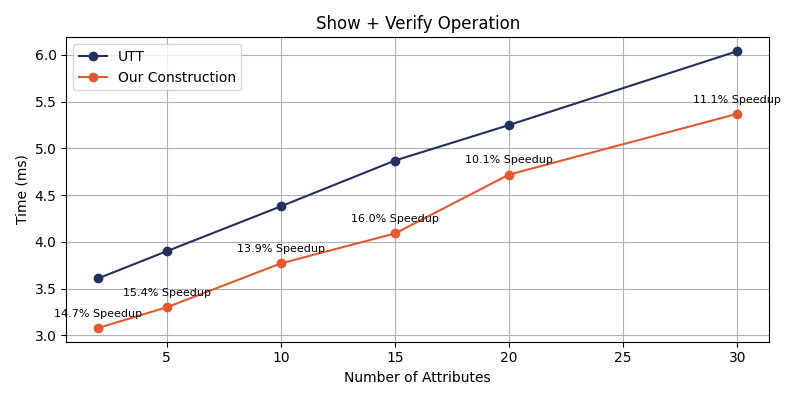
\includegraphics[width=0.75\textwidth]{figures/show_verify_utt_g2.png}
    \end{minipage}
    
    \vspace{0.05cm}

    \vspace{0.05cm}
    
    % Bottom row with 2x2 grid of smaller figures
    \begin{minipage}{0.48\textwidth}
        \centering
        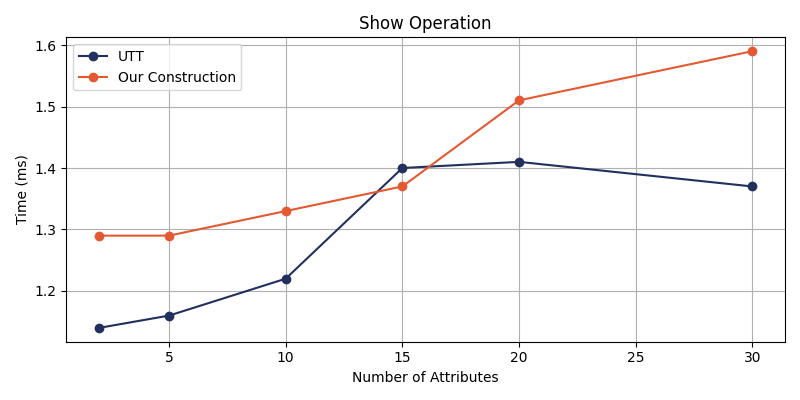
\includegraphics[width=\textwidth]{figures/show_utt_g2.png}
    \end{minipage}
    \hfill
    \begin{minipage}{0.48\textwidth}
        \centering
        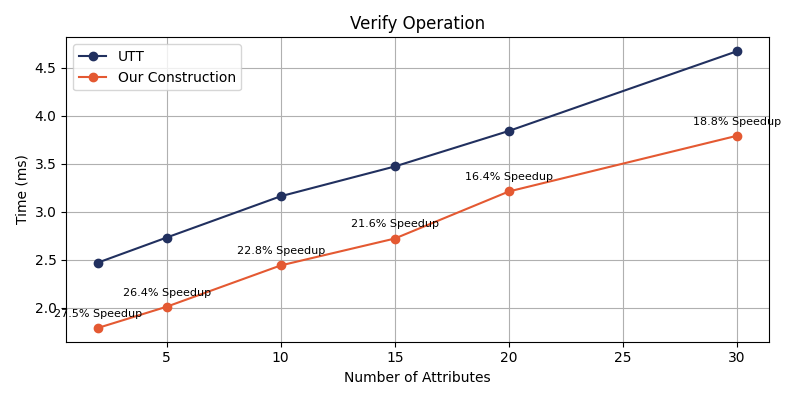
\includegraphics[width=\textwidth]{figures/verify_utt_g2.png}
    \end{minipage}
    
    \caption{Performance Comparison between UTT and Our Construction. We improve key operations: Verify and Show + Verify}
    \label{fig:show_verify_utt_us}
\end{figure}



\begin{table}[htbp]
\centering
\caption{Performance Comparison: PS-UTT and Our Construction (time in ms)}
\label{tab:g1-g2-comparison}
\begin{tabular}{l@{\hspace{1em}}r@{\hspace{1.5em}}r@{\hspace{2em}}r@{\hspace{1.5em}}r@{\hspace{2em}}r@{\hspace{1.5em}}r}
\toprule
\textbf{Attributes} & \multicolumn{2}{c@{\hspace{4em}}}{\textbf{Show}} & \multicolumn{2}{c@{\hspace{2.5em}}}{\textbf{Verify}} & \multicolumn{2}{c}{\textbf{Show + Verify}} \\
\cmidrule(lr){2-3} \cmidrule(lr){4-5} \cmidrule(lr){6-7}
 & \textbf{G1} & \textbf{G2 (Ours)} & \textbf{G1} & \textbf{G2 (Ours)} & \textbf{G1} & \textbf{G2 (Ours)} \\
\midrule
2 & 1.14 & 1.29 (11.6\% $\uparrow$) & 2.47 & 1.79 (27.5\% $\downarrow$) & 3.61 & 3.08 (14.7\%$\downarrow$) \\
5 & 1.16 & 1.29 (10.1\% $\uparrow$)& 2.73 & 2.01 (26.4\%$\downarrow$) & 3.90 & 3.30 (15.4\%$\downarrow$) \\
10 & 1.22 & 1.33 (8.27\% $\uparrow$) & 3.16 & 2.44 (22.8\%$\downarrow$) & 4.38 & 3.77 (13.9\%$\downarrow$) \\
15 & 1.40 & 1.37 (2.19\% $\downarrow$)& 3.47 & 2.72 (21.6\%$\downarrow$) & 4.87 & 4.09 (16.0\%$\downarrow$) \\
20 & 1.41 & 1.51 (6.62\% $\uparrow$) & 3.84 & 3.21 (16.4\%$\downarrow$) & 5.25 & 4.72 (10.1\%$\downarrow$) \\
30 & 1.37 & 1.59 (13.8\% $\uparrow$)& 4.67 & 3.79 (18.8\%$\downarrow$) & 6.04 & 5.37 (11.1\%$\downarrow$) \\
\bottomrule
\end{tabular}
\end{table}





\subsection{Performance Comparison: Our Construction is State-Of-The-Art}

We now present a comprehensive comparison of our construction against four state-of-the-art anonymous credential schemes. Table~\ref{abc-performance-combined-table} summarizes the performance across all credential operations and attribute counts.

\begin{figure}
    \centering
    % First row with two larger figures
    \begin{minipage}{\textwidth}
        \centering
        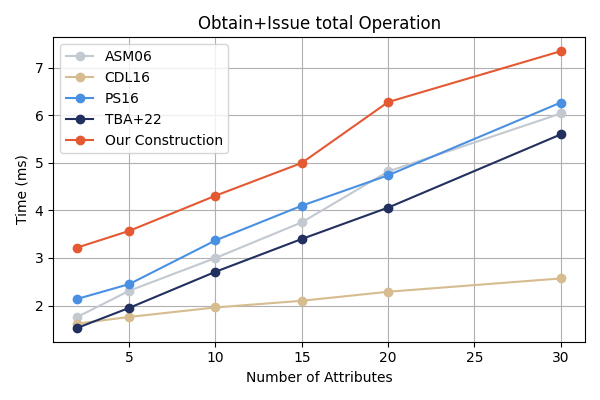
\includegraphics[width=0.75\textwidth]{figures/anoncreds_obtain_issue.png}
    \end{minipage}
    
    \vspace{0.05cm}
    
    \begin{minipage}{\textwidth}
        \centering
        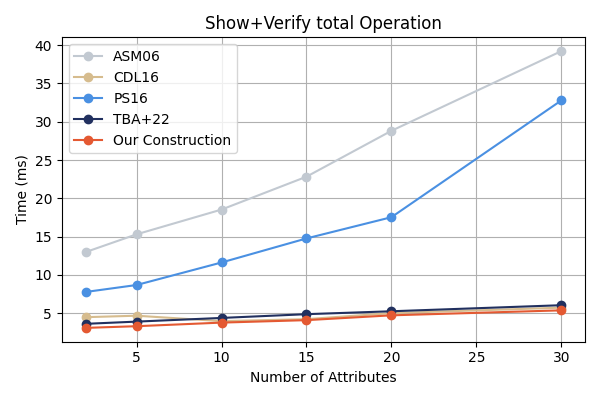
\includegraphics[width=0.75\textwidth]{figures/anoncreds_show_verify.png}
    \end{minipage}
    
    \vspace{0.05cm}
    
    % Bottom row with 2x2 grid of smaller figures
    \begin{minipage}{0.48\textwidth}
        \centering
        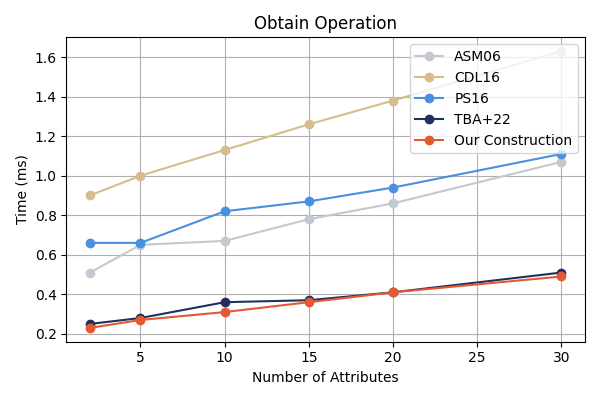
\includegraphics[width=\textwidth]{figures/anoncreds_obtain.png}
    \end{minipage}
    \hfill
    \begin{minipage}{0.48\textwidth}
        \centering
        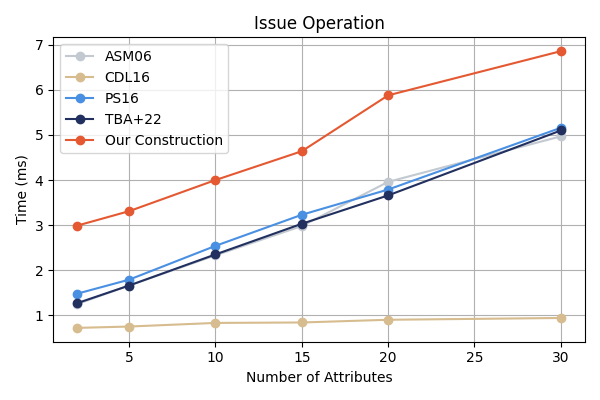
\includegraphics[width=\textwidth]{figures/anoncreds_issue.png}
    \end{minipage}
    
    \vspace{0.1cm}
    
    \begin{minipage}{0.48\textwidth}
        \centering
        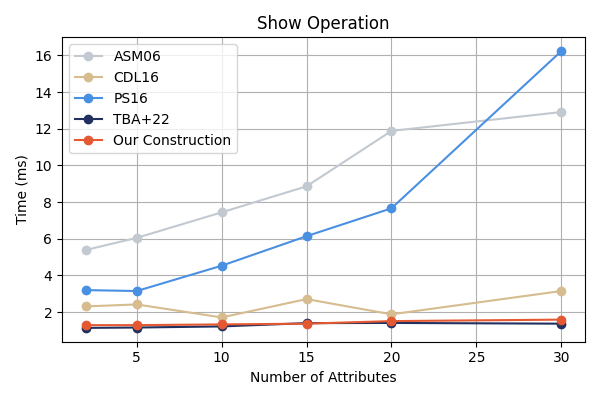
\includegraphics[width=\textwidth]{figures/anoncreds_show.png}
    \end{minipage}
    \hfill
    \begin{minipage}{0.48\textwidth}
        \centering
        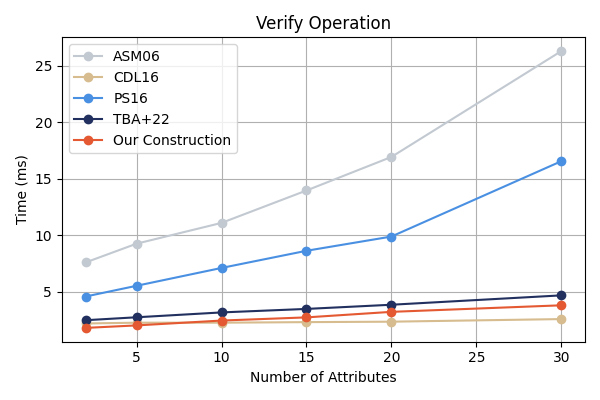
\includegraphics[width=\textwidth]{figures/anoncreds_verify.png}
    \end{minipage}
    
    \caption{Performance comparison of different operations across varying numbers of attributes}
    \label{fig:anoncreds-performance}
\end{figure}

\begin{table}[htbp]\label{abc-performance-combined-table}
\centering
\caption{Performance of Anonymous Credential Operations (time in ms), $n$ is attribute count}
\begin{tabular}{@{}p{1.2cm}*{5}{>{\centering\arraybackslash}p{1.6cm}}@{}}
\toprule
$n$ & \cite{hutchison_constant-size_2006} & \cite{camenisch_anonymous_2016} & \cite{sako_short_2016} & \cite{tomescu_utt_2022} \ref{subsec:g2_verify_speedup} & Our Construction \\
\midrule
\multicolumn{6}{c}{\textbf{Obtain}}  \\
\midrule
\textbf{2} & 0.51 & 0.90 & 0.66 & 0.25 & \textbf{0.23} \\
\textbf{5} & 0.65 & 1.00 & 0.66 & 0.28 & \textbf{0.27} \\
\textbf{10} & 0.67 & 1.13 & 0.82 & 0.36 & \textbf{0.31} \\
\textbf{15} & 0.78 & 1.26 & 0.87 & 0.37 & \textbf{0.36} \\
\textbf{20} & 0.86 & 1.38 & 0.94 & \textbf{0.41} & \textbf{0.41} \\
\textbf{30} & 1.07 & 1.63 & 1.11 & 0.51 & \textbf{0.49} \\
\midrule
\multicolumn{6}{c}{\textbf{Issue}}  \\
\midrule
\textbf{2} & 1.25 & \textbf{0.72} & 1.48 & 1.27 & 2.99 \\
\textbf{5} & 1.66 & \textbf{0.75} & 1.79 & 1.66 & 3.31 \\
\textbf{10} & 2.33 & \textbf{0.83} & 2.54 & 2.35 & 4.00 \\
\textbf{15} & 2.98 & \textbf{0.84} & 3.23 & 3.03 & 4.64 \\
\textbf{20} & 3.96 & \textbf{0.90} & 3.79 & 3.66 & 5.88 \\
\textbf{30} & 4.97 & \textbf{0.94} & 5.16 & 5.10 & 6.86 \\
\midrule
\multicolumn{6}{c}{\textbf{Show}}  \\
\midrule
\textbf{2} & 5.39 & 2.31 & 3.20 & \textbf{1.14} & 1.29 \\
\textbf{5} & 6.05 & 2.42 & 3.15 & \textbf{1.16} & 1.29 \\
\textbf{10} & 7.44 & 1.71 & 4.53 & \textbf{1.22} & 1.33 \\
\textbf{15} & 8.86 & 2.71 & 6.14 & 1.40 & \textbf{1.37} \\
\textbf{20} & 11.88 & 1.88 & 7.66 & \textbf{1.41} & 1.51 \\
\textbf{30} & 12.91 & 3.15 & 16.23 & \textbf{1.37} & 1.59 \\
\midrule
\multicolumn{6}{c}{\textbf{Verify}}  \\
\midrule
\textbf{2} & 7.59 & 2.18 & 4.57 & 2.47 & \textbf{1.79} \\
\textbf{5} & 9.25 & 2.25 & 5.52 & 2.73 & \textbf{2.01} \\
\textbf{10} & 11.09 & \textbf{2.25} & 7.10 & 3.16 & 2.44 \\
\textbf{15} & 13.96 & \textbf{2.30} & 8.62 & 3.47 & 2.72 \\
\textbf{20} & 16.93 & \textbf{2.34} & 9.88 & 3.84 & 3.21 \\
\textbf{30} & 26.30 & \textbf{2.57} & 16.55 & 4.67 & 3.79 \\
\midrule
\multicolumn{6}{c}{\textbf{Issuing Phase Total (Obtain + Issue)}}  \\
\midrule
\textbf{2} & 1.76 & 1.62 & 2.14 & \textbf{1.53} & 3.22 \\
\textbf{5} & 2.31 & \textbf{1.76} & 2.45 & 1.95 & 3.57 \\
\textbf{10} & 3.00 & \textbf{1.96} & 3.37 & 2.71 & 4.31 \\
\textbf{15} & 3.75 & \textbf{2.10} & 4.10 & 3.40 & 5.00 \\
\textbf{20} & 4.82 & \textbf{2.29} & 4.74 & 4.06 & 6.28 \\
\textbf{30} & 6.04 & \textbf{2.57} & 6.27 & 5.60 & 7.35 \\
\midrule
\multicolumn{6}{c}{\textbf{Showing Phase Total (Show + Verify)}}  \\
\midrule
\textbf{2} & 12.98 & 4.48 & 7.77 & 3.61 & \textbf{3.08} \\
\textbf{5} & 15.30 & 4.67 & 8.68 & 3.90 & \textbf{3.30} \\
\textbf{10} & 18.53 & 3.96 & 11.62 & 4.38 & \textbf{3.77} \\
\textbf{15} & 22.82 & 4.22 & 14.76 & 4.87 & \textbf{4.09} \\
\textbf{20} & 28.81 & 5.01 & 17.53 & 5.25 & \textbf{4.72} \\
\textbf{30} & 39.21 & 5.72 & 32.77 & 6.04 & \textbf{5.37} \\
\bottomrule
\end{tabular}
\end{table}

\subsubsection{Key Findings}
\begin{enumerate}
    \item \textbf{Optimized}: Our PS-UTT G2 variant achieves the best Show+Verify performance (10-16\% faster than PS-UTT G1 and up to 83\% faster than BBS+ 2006), optimizing the operation that occurs most frequently in practice. While the Issue operation is more costly, credentials are issued once but verified many times.
    
    \item \textbf{Evolution of Efficiency}: The original constructions \cite{hutchison_constant-size_2006, sako_short_2016} required proof of knowledge for $\mathbb{G}_T$ points, resulting in slower operations. Later optimizations \cite{camenisch_anonymous_2016, tomescu_utt_2022} shifted proof of knowledge work to $\G_1$ reducing Show+Verify time by up to 6x. 
    
    \item \textbf{Favorable Scaling Properties}: While all schemes exhibit approximately linear scaling with attribute count, our PS-UTT G2 is the most efficient.
\end{enumerate}




\subsection{Future Work}
Benchmark these schemes against SPS-EQ and zk-creds for efficient anonymous credential comparison.


































% \subsection{Introduction}
% Privacy-preserving authentication systems require cryptographic primitives that allow users to prove certified attributes (e.g., citizenship, qualifications) without revealing additional information or enabling linkage across sessions. Anonymous credential schemes address this by encoding attributes into cryptographically randomized signatures, enabling users to generate unlinkable "showings" of credentials through zero-knowledge proofs (ZKPs). A critical challenge lies in balancing three properties: (1) multi-show unlinkability (proving attributes without correlating sessions), (2) selective disclosure (revealing subsets of attributes), and (3) practical efficiency for real-world deployment.

% The problems in accountable privacy were first introduced by Chaum \cite{chaum_untraceable_1981, chaum1985security} and later formalized as the \emph{CL framework} \cite{goos_pseudonym_2000, goos_efficient_2001}, establishing the paradigm of encoding credentials as signatures over committed attributes. While early signature schemes lacked the algebraic structure to support efficient ZKPs and signature randomization, the advent of pairing-based cryptography \cite{goos_short_2001, hutchison_short_2004} coupled with commitment schemes and zero-knowledge proof systems enabled homomorphic rerandomization of credentials—allowing users to transform signatures into fresh, unlinkable versions while preserving validity.

% \subsection{Evolution of Anonymous Credential Schemes}
% The progression of anonymous credential schemes reflects a sustained effort to simplify the mathematical structures underlying zero-knowledge proofs:

% \paragraph{CL Signatures \cite{cimato_signature_2003, hutchison_signature_2004}}
% Built on early pairing-based constructions, CL credentials introduced homomorphic rerandomization but required linear-in-attributes pairing operations during proofs, limiting scalability for complex credentials.

% \paragraph{BBS+ Signatures \cite{hutchison_constant-size_2006}}
% Achieved constant-size credentials by intertwining message commitments with signatures. While \cite{camenisch_anonymous_2016} improved computational complexity, The signature leverages the q-SDH assumption \cite{boneh_short_2008}, requiring a mathematical structure that which intertwines the message and secret key $A^{\frac{1}{x+e}}$ which enables zkp statements but complicates proofs 

% \paragraph{BBS+ Signatures \cite{hutchison_constant-size_2006}}
% Achieved constant-size credentials through a structure where signatures take the form $A = (gh_0^s\prod_{i=1}^n h_i^{m_i})^{\frac{1}{e+x}}$. While \cite{camenisch_anonymous_2016} improved computational complexity, the signature structure necessitates complex blinding operations with inverse relationships ($r_3 = \frac{1}{r_1}$), cross-terms ($s' = s - r_2 \cdot r_3$), and complex equality checks during proof generation, e.g. 
% \[
% g = ((gh_0^s \prod_1^nh_i^{-m_i})^{r_1} \cdot h_0^{-r_2})^{r_3}h_0^{-s'}\prod_{i=1}^n h_i^{-m_i}
% \]
% This leads to a zero-knowledge proof relation involving multiple auxiliary variables and non-linear equations, complicating the implementation and composition of proofs across multiple credentials.


% \paragraph{PS and PS\_UTT Signatures \cite{sako_short_2016, tomescu2022utt}}
% Introduced separation between signature components and message commitments. The UTT variant further simplified rerandomization by decoupling attribute commitments from the core signature structure, enabling linear ZKP relations over Pedersen commitments. PS based signature rely on the LRSW assumption \cite{goos_pseudonym_2000} rather than BBS+ q-SDH which enables simpler algebraic structures, which we show now. 

% \subsection{Cryptographic Foundations: q-SDH vs LRSW}
% The choice between these shapes the proof complexity:

% \paragraph{BBS+ and q-SDH Limitations}
% The $q$-Strong Diffie-Hellman (q-SDH) assumption \cite{boneh_short_2008} requires signatures of the form $A = (g_0g_1^s\prod h_i^{m_i})^{\frac{1}{e+x}}$. This structure:
% \begin{itemize}
%     \item Demands \textit{inverse exponentiation} ($1/(e+x)$), creating non-linear relationships between secrets
%     \item Forces proofs to handle \textit{cross-term cancellation} (e.g., $A_1^e = g_1^{\delta_1}g_2^{\delta_2}$)
%     \item Requires pairing inversions ($e(A_2, \hat{h_0})^{-e}$) to verify credential validity
% \end{itemize}


% \paragraph{PS\_UTT and LRSW Advantages}
% The LRSW assumption \cite{lysyanskaya2000pseudonym} underpinning PS\_UTT enables signatures with \textit{linear} algebraic structure:
% \begin{itemize}
%     \item Signatures take form $\sigma = (h^u, (X \cdot \prod g_i^{m_i} \cdot h^r)^u)$ with \textit{no inverse operations}
%     % \item Randomization factors ($u_\Delta, r_\Delta$) modify signatures additively rather than multiplicatively
%     \item Verification equations remain bilinear pairings without cross-term cancellation
% \end{itemize}


% \paragraph{Assumption-Driven Efficiency}
% The LRSW assumption enables three key efficiency properties, each building on the previous:
% \begin{itemize}
%     \item \textbf{Linear Exponent Relations}: Messages appear directly in the exponent as $\prod g_i^{m_i}$, avoiding the nested fraction structure of q-SDH
%     \item \textbf{Independent Randomization}: The separation of $u_\Delta$ and $r_\Delta$ creates a natural two-layer randomization strategy, unlike BBS+'s entangled randomized
% \end{itemize}



% \begin{figure}
%     \centering
% \begin{pcvstack}[boxed]
%         \procedure[linenumbering]{$\mathrm{Sim}^{\mathsf{\UNF}}_{\MIMCABC, \adv}(\lambda)$}{%
%             \AdvB \text{ Setup Simulation  } \\
%             \vk \gets \text{Challenge from } \EUFCMA \text{ game from $\RS$} \\
%             \ck \gets \text{Challenge from } \POSBINDING \text{ game from $\CM$} \\
%             \AdvB \text{ Embeds $\vk, \ck$ into $\MIMCABC$ public params $\pp$ and issuer keys $\{\opk_j\}$} \\
%             \text{Simulating $\mathrm{Game}^{\mathsf{UNF}_{\MIMCABC}}$ setup for $\AdvA$} 
%             \\
%             \AdvB \text{ uses real $\OHU, \OCU$ and simulates $\OOBTAIN, \OSHOW$} \\
%             \AdvA \text{ outputs forgery } \{ \cred_k'^*, \phi^*, \pi^* \} \\
%             \AdvB \text{ processes the forgery to break the assumption}
%         }
%         \procedure[]{$\AdvB$ Simulates $\OOBTAIN(i, j, \vec{m})$}{%
%             \pcif i \notin \HU, \pcreturn \bot \quad \greyt{// Only honest users can obtain credentials} \\
%             \t \usk \gets \mathbb{Z}_p \quad \greyt{// Generate fresh randomness for commitment} \\
%             \t \cm \gets \CMCom(\vec{m}; \usk) \quad \greyt{// Commitment to attributes} \\
%             \t \pcif j \neq j^*, \\
%             \t \t \sigma \gets \RSSign(\osk_j, \cm) \quad \greyt{// Sign using known issuer key} \\
%             \t \pcelse \quad \greyt{// Case: } j = j^* \\
%             \t \t \sigma \gets \OEUFCMA(\cm) \quad \greyt{// Query EUF-CMA oracle for signature} \\
%             \t \cred \gets (\sigma, \cm) \quad  \\
%             \t \CRED_j \gets \CRED_j \cup \{(\cred, \cm, \vec{m}, \usk, i)\} \\
%             \t \OWNR[\cred] \gets i \\
%             \pcreturn \cred
%         }
%         \procedure[]{$\AdvB$ Simulates $\OSHOW(i, \phi)$}{%
%             \pcif i \notin \HU, \pcreturn \bot \quad \greyt{// Only honest users can show proofs} \\
%             \t \text{Let } \creds_i \text{ be the credentials of user } i \text{ in } \HU \\
%             \t \pcif \phi(\text{attributes in } \creds_i) = 0, \pcreturn \bot \quad \greyt{// Check policy satisfaction} \\
%             \t \pi \gets \text{ZKSim}(\phi, \{ \cred_k' \}, \{ \cm_k' \}, \text{ Simulate proof without witness})\\
%             \SHOW \gets \SHOW \cup (i, \phi, \pi) \\
%             \pcreturn \pi
%         }
%     \end{pcvstack}
%     \caption{Simulated Oracles}
    
% \end{figure}

